%% =====================================================================================
%%  Working paper -- build of the note until a target outlet is chosen
%% -------------------------------------------------------------------------------------
%%  Only layout settings belong here: class, page geometry, links, bibliography style.
%%  The note's content lives in ../../manuscript/ and is shared by every wrapper.
%%  Keep the relative \input paths literal.
%%
%%  Build:  cd journals/working-paper && latexmk main.tex
%%     or:  latexmk main.tex from the repository root (as Overleaf does; see the root main.tex)
%%  Clean PDF without drafting markers: define \FinalVersion before \documentclass.
%% =====================================================================================
\documentclass[11pt,a4paper]{article}

%% ------------------------------------------------------------------------------------------------
%%  Packages the content needs. Journal-agnostic: no page layout, class or bibliography style here
%%  (those live in journals/<journal>/main.tex).
%% ------------------------------------------------------------------------------------------------
\usepackage[utf8]{inputenc}
\usepackage[T1]{fontenc}
\usepackage{lmodern}
\usepackage{amsmath,amssymb,amsthm}
\usepackage{graphicx}
\usepackage{booktabs,array}             % generated tables in outputs/tables/ need both
\usepackage{tabularx}
\usepackage{caption}
%% Captions: a short title in the caption; notes and source under the table or figure, smaller
%% (\figurenotes for figures, \tabnotes for tables).
\captionsetup{font=small,labelfont=bf,labelsep=period,skip=4pt}
\captionsetup[table]{position=top}
\captionsetup[figure]{position=bottom}
\usepackage{xcolor}
\usepackage[authoryear,round]{natbib}
\usepackage{authblk}
\usepackage{url}
\Urlmuskip=0mu plus 1mu                 % let long URLs in the references stretch and break
\expandafter\def\expandafter\UrlBreaks\expandafter{\UrlBreaks\do\-}
\usepackage{enumitem}
\setlist{itemsep=1pt,topsep=3pt}
\usepackage{algorithm}
\usepackage{algpseudocode}              % the procedure, Algorithm 1


%% ---- Layout ----------------------------------------------------------------------------
\usepackage[margin=25mm]{geometry}
\setlength{\parskip}{0.3\baselineskip}
\numberwithin{equation}{section}
\renewcommand\Affilfont{\itshape\small}
\usepackage[colorlinks,linkcolor=blue,citecolor=blue,urlcolor=blue]{hyperref}

%% ------------------------------------------------------------------------------------------------
%%  Notation and drafting macros. Journal-agnostic.
%% ------------------------------------------------------------------------------------------------

%% ---- Notation ----------------------------------------------------------------------------------
\newcommand{\Voters}{N}                 % the voters, n = |N|
\newcommand{\Opts}{A}                   % the options, m = |A|, the status quo s included
\newcommand{\sq}{s}                     % the status quo
\newcommand{\pref}{\succ}               % strict preference of a voter
\newcommand{\wpref}{\succsim}           % weak preference
\newcommand{\Maj}{\operatorname{N}}     % N(x,y): number of voters who prefer x to y
\newcommand{\veto}{v}                   % v(x): number of voters who veto x
\newcommand{\Adm}{A_\theta}             % admissible options under the blocking quota theta
\newcommand{\QVC}{\textup{QVC}}         % Condorcet with a blocking quota
\newcommand{\PVC}{\textup{PVC}}         % proportional veto core
\newcommand{\E}{\mathbb{E}}
\newcommand{\Prob}{\mathbb{P}}
\newcommand{\conv}{\operatorname{conv}}
\newcommand{\Normal}{\mathcal{N}}

%% ---- Notes of figures and tables ------------------------------------------------------------------
%% \figurenotes{notes}{source}  after \caption{title} in a figure: the notes and the source, smaller
%% \tabnotes{notes}{source}     after a tabular boxed in \tabbox (generated tables): the same, as wide as
%%                              the table but not narrower than 70% of the text
\newcommand{\figurenotes}[2]{\par\vspace{3pt}%
  {\footnotesize\raggedright\textit{Notes:} #1\par\textit{Source:} #2\par}}
\newsavebox{\tabbox}
\newlength{\tabnoteswidth}
\newcommand{\tabnotes}[2]{\par\vspace{3pt}%
  \setlength{\tabnoteswidth}{\wd\tabbox}%
  \ifdim\tabnoteswidth<0.7\linewidth\setlength{\tabnoteswidth}{0.7\linewidth}\fi
  \ifdim\tabnoteswidth>\linewidth\setlength{\tabnoteswidth}{\linewidth}\fi
  \begin{minipage}{\tabnoteswidth}\footnotesize\raggedright
  \textit{Notes:} #1\par\textit{Source:} #2\end{minipage}\par}

%% ---- Drafting markers ----------------------------------------------------------------------------
%% \placeholder{...}  work still to do (shown in red; must be empty before circulation)
%% \prelim{...}       a number to update when the simulation is extended (shown in orange)
%% Define \FinalVersion before \documentclass to hide the markers (as in Immo_S2).
\definecolor{placeholdercolor}{rgb}{0.75,0.0,0.0}
\definecolor{prelimcolor}{rgb}{0.85,0.45,0.0}
\ifdefined\FinalVersion
  \newcommand{\placeholder}[1]{}
  \newcommand{\prelim}[1]{#1}
\else
  \newcommand{\placeholder}[1]{\textcolor{placeholdercolor}{\textbf{[To do:} #1\textbf{]}}}
  \newcommand{\prelim}[1]{\textcolor{prelimcolor}{#1}}
\fi

%% ------------------------------------------------------------------------------------------------
%%  Theorem-like environments. Journal-agnostic.
%% ------------------------------------------------------------------------------------------------
\theoremstyle{plain}
\newtheorem{proposition}{Proposition}
\newtheorem{corollary}[proposition]{Corollary}
\newtheorem{lemma}[proposition]{Lemma}
\theoremstyle{definition}
\newtheorem{definition}{Definition}
\newtheorem{assumption}{Assumption}
\newtheorem{example}{Example}
\theoremstyle{remark}
\newtheorem{remark}{Remark}

%% ------------------------------------------------------------------------------------------------
%%  Title, authors, affiliations. Journal-agnostic.
%% ------------------------------------------------------------------------------------------------
\title{Voting for a consensus with veto rights: a state-of-the-art note\\[4pt]
\large Open proposals, full ballots and a blocking quota}

\author[1]{Fabrice Borel-Mathurin}
\affil[1]{Draft for discussion}
\date{\today}


%% Static figures, then figures generated by simulations/. The first two paths serve a build in this folder,
%% the last two a build from the repository root (Overleaf), which does not rely on latexmkrc for them.
\graphicspath{{../../manuscript/figures/}{../../outputs/figures/}{manuscript/figures/}{outputs/figures/}}

%% The bibliography file, relative to the folder LaTeX runs in: this folder by default; the root main.tex
%% redefines it for a build from the repository root.
\providecommand{\NoteBibliography}{../../manuscript/references}

\begin{document}
\maketitle
%% ------------------------------------------------------------------------------------------------
%%  Abstract and keywords. Journal-agnostic.
%% ------------------------------------------------------------------------------------------------
\begin{abstract}
A group wants to choose one option by consensus. Anyone may propose options, every voter judges all of
them, and voters have a right of veto. We review what research says about voting in this setting and
derive a procedure that reaches the best compromise without ever getting stuck. The literature on
committees, veto players and consensus practice agrees that hard unanimity is rarely optimal: it breeds
delay, status-quo bias and holdouts, and in a large assembly it deadlocks almost surely, as we show for
spatial preferences. Social choice adds three constraints: no rule escapes manipulation, the majority
principle and a minority veto conflict in some profiles, and an open agenda requires a rule that is
independent of clones, which Borda's rule, fallback bargaining and the proportional veto core are not. We
propose \emph{Condorcet with a blocking quota}: on a single ballot, every voter ranks all options and marks
the unacceptable ones; options vetoed by at least a third of the voters are excluded, the least-vetoed are
kept if all are, and the Schulze winner among the rest is elected. The procedure always decides in one
round, gives the status quo no default advantage, elects an option acceptable to more than two thirds of
the voters whenever one exists, respects the majority among such options and ignores clones. In
simulations of polarised electorates it halves the share of contested outcomes relative to the Schulze
method, at no cost in total welfare. Its price is strategic blocking, which we quantify and which named,
reasoned vetoes and a bounded revision round help contain.

\medskip
\noindent\textbf{Keywords.} Voting rules, veto rights, consensus, Condorcet methods, Schulze method,
independence of clones, proportional veto, deadlock, compromise.
\end{abstract}

\tableofcontents
%% ------------------------------------------------------------------------------------------------
%%  Body of the note: section order. Paths are relative to the journal wrapper
%%  (journals/<journal>/main.tex), which is where LaTeX runs.
%% ------------------------------------------------------------------------------------------------
%% ================================================================================================
%%  1. Introduction
%%  Notes: research-agenda.md §0 (question, hypotheses, requirements), §1 (answer in brief)
%% ================================================================================================
\section{Introduction}\label{sec:intro}

\subsection{The question}

A group has to choose one option among several: a site, a design, a budget allocation, a policy. The
group wants a \emph{consensus} choice, one that everyone can live with, and it wants a procedure that
produces one. This note asks what the research literature says about the optimal way to vote in that
situation, and turns the answer into a procedure that can be implemented. We work under three
hypotheses, set by the use case:
\begin{description}
  \item[H1 (open agenda)] any voter may propose as many options as they wish;
  \item[H2 (full ballots)] every voter expresses a view on \emph{all} the options proposed;
  \item[H3 (veto rights)] voters have a right of veto.
\end{description}
The procedure must meet two requirements:
\begin{description}
  \item[R1 (best compromise)] the option chosen is the best compromise, in a sense to be made precise;
  \item[R2 (no deadlock)] the community never gets stuck, so the veto must not be too stringent.
\end{description}

The two requirements pull against each other. The traditional consensus rule, unanimity, gives every
member a veto: nothing passes to which anyone objects. It protects every minority, which is the spirit
of R1, but a single objector can block every change, and in large or divided groups someone always
objects (Section~\ref{sec:limits}). The Polish--Lithuanian \emph{liberum veto} is the textbook
case of a constitution paralysed by individual vetoes \citep{Rohac2008}. Majority rule, at the other
extreme, always decides (R2) but can impose on a large minority an outcome it finds unacceptable, which
is not a compromise. The question is therefore one of design: how much veto power, held by whom, over
what, and how to aggregate the rest of the ballot.

\subsection{The answer in brief}

\begin{enumerate}
  \item \textbf{No rule is optimal in every respect.} Every rule that is not dictatorial can be
  manipulated \citep{Gibbard1973,Satterthwaite1975}, majorities can cycle \citep{Condorcet1785}, and
  the majority principle cannot be reconciled with an effective minority veto: some profiles force a
  choice between the option a majority prefers and the one a large minority can accept
  (Proposition~\ref{prop:majority-veto}). A procedure is a choice of trade-off, which should be explicit
  and tunable.
  \item \textbf{The literature does not support hard unanimity.} Theory, experiments and institutional
  studies agree that unanimity raises delay, strengthens the status quo and gives holdouts bargaining
  power. Veto rights work better when they are separated from the approval of options and limited to
  blocking outcomes that are unacceptable
  \citep{BoutonLlorenteSaguerMalherbe2018,MiettinenVanberg2025,Tsebelis2002,DziudaLoeper2016}. In a large
  assembly, unanimity with the status quo as default deadlocks almost surely
  (Proposition~\ref{prop:gridlock}; 99.6\% of our simulated elections with 101 voters).
  \item \textbf{An open agenda requires a rule that is independent of clones.} When anyone can add
  options, a faction can flood the agenda with variants of its favourite. Borda's rule, fallback
  bargaining and the proportional veto core reward such flooding; the Schulze, Ranked Pairs and Split
  Cycle methods do not \citep{Tideman1987,Schulze2011,HollidayPacuit2023splitcycle}.
  \item \textbf{The procedure we recommend, \QVC($\theta$)}, Condorcet with a blocking quota, uses a
  single ballot on which each voter ranks all the options and marks those they find unacceptable.
  Options vetoed by at least a share $\theta$ of the voters are excluded; if that excludes them all, the
  least-vetoed are kept; the Schulze winner among the options left is elected. By default
  $\theta = 1/3$. The procedure always decides in one round, the status quo has no default advantage, the
  winner is acceptable to more than two thirds of the voters whenever some option is, the option that
  beats every other acceptable option in pairwise majority wins, and adding variants of an option changes
  nothing (Section~\ref{sec:procedure}).
  \item \textbf{The price is strategic vetoing.} A blocking minority can block strategically as well as
  sincerely. In our simulations, the share of elections that a coalition of 10\% of the voters can
  manipulate rises from 5--7\% under Schulze to 11--27\% under \QVC(1/3) in structured electorates
  (Section~\ref{sec:simulation}). Named and reasoned vetoes, a quota no lower than $1/4$ and at most one
  revision round contain this risk (Section~\ref{sec:safeguards}).
\end{enumerate}

\subsection{What this note adds and how it is organised}

The note starts from a literature review of optimal voting with veto rights produced with the
Consensus search engine in October 2026 (summarised in the repository's \texttt{literature/} folder). That
review covers committee bargaining and the comparison of unanimity with majority-with-veto. We add the
social-choice literature on Condorcet methods, clones and proportional veto, the evidence from
institutions that already vote this way, formal results on deadlock and on the procedure, and a Monte
Carlo study of 21 rules on 2,000 simulated elections per setting. Every number in the note comes from
code in the repository (\texttt{simulations/python/}), with checks against known results.

Section~\ref{sec:setting} sets out the model and the definitions. Section~\ref{sec:limits} states what
no procedure can achieve. Section~\ref{sec:veto} reviews the research on veto rights,
Section~\ref{sec:aggregation} the rules that aggregate full ballots. Section~\ref{sec:procedure} defines
and analyses the procedure, Section~\ref{sec:simulation} compares it with the alternatives by
simulation, and Section~\ref{sec:discussion} discusses limits, open questions and implementation.
Proofs are in Appendix~\ref{app:proofs}, algorithms in Appendix~\ref{app:algorithms} and the details of
the simulation in Appendix~\ref{app:simulation}.

%% ================================================================================================
%%  2. Setting and definitions
%%  Notes: research-agenda.md §2; code: simulations/python/voting.py (Election, rules)
%% ================================================================================================
\section{Setting and definitions}\label{sec:setting}

\subsection{Voters, options and ballots}

A finite set $\Voters$ of $n$ voters chooses one option from a finite set $\Opts$ of $m$ options. The
set $\Opts$ is the union of the proposals made by the voters during a nomination period (H1), plus the
status quo $\sq$, which stands for ``keep things as they are'' or ``no decision'' and is treated as an
option. Each voter casts one ballot on all the options (H2) with two parts:
\begin{itemize}
  \item a \emph{ranking}: a weak order $\wpref_i$ on $\Opts$ (ties allowed), whose strict part is
  $\pref_i$;
  \item a \emph{veto set} $V_i \subseteq \Opts$ of options the voter finds unacceptable (H3). The veto
  set is consistent with the ranking: if $x \in V_i$ and $x \wpref_i y$, then $y \in V_i$. A ballot is
  thus a ranking with an \emph{acceptability line} drawn in it, as in fallback bargaining with
  impasse \citep{BramsKilgour2001}, in Majority Judgment's ``reject'' grade \citep{BalinskiLaraki2011},
  or in Debian's ranking of options above or below the default option \citep{Debian2024constitution}.
\end{itemize}
We write $\Maj(x,y) = |\{i : x \pref_i y\}|$ for the number of voters who prefer $x$ to $y$, and
$\veto(x) = |\{i : x \in V_i\}|$ for the number of voters who veto $x$. A \emph{rule} maps every
profile of ballots to one option; rules that return a set of tied options are completed by a
tie-breaking rule.

\subsection{Majority relations}

\begin{definition}[Condorcet winner, Smith set]\label{def:condorcet}
Option $x$ \emph{beats} $y$ if $\Maj(x,y) > \Maj(y,x)$. A \emph{Condorcet winner} beats every other
option. The \emph{Smith set} is the smallest non-empty set of options each of which beats every option
outside it \citep{Smith1973,Fishburn1977}. A rule is \emph{Condorcet-consistent} if it elects the
Condorcet winner whenever one exists, and \emph{Smith-consistent} if it always elects an option of the
Smith set.
\end{definition}

The Condorcet winner is the natural majoritarian notion of a compromise: whatever other option is put
against it, a majority prefers it. It need not exist (the Condorcet paradox), and when it exists it
need not protect minorities (Section~\ref{sec:limits}).

\subsection{Properties a procedure should have}

\begin{definition}[Clones; \citealp{Tideman1987}]\label{def:clones}
A set $C \subseteq \Opts$ with at least two options is a set of \emph{clones} if no voter ranks an
option outside $C$ between two options of $C$ or level with one of them, and every voter vetoes either
all the options of $C$ or none. A rule is \emph{independent of clones} if, whenever a clone of an option
is added or removed, (i) an option outside the clone set wins after the change if and only if it won
before, and (ii) a member of the clone set wins after the change if and only if one won before.
\end{definition}

Clones are variants of the same proposal: two near-identical sites, a budget and the same budget with
one line moved. Under H1 anyone can create them, so independence of clones is what makes a rule robust
to flooding the agenda.

\begin{definition}[Decisiveness]\label{def:decisive}
A procedure is \emph{decisive} if, for every profile, it selects one option after a number of rounds
fixed in advance. It gives the status quo \emph{no default advantage} if the status quo is selected only
when it would also be selected with its label removed, as an ordinary option.
\end{definition}

R2 asks for decisiveness. A procedure that keeps the status quo whenever no proposal clears a hurdle is
decisive in a formal sense, but it gets the community stuck whenever the status quo is not what the
voters want; this is why we also ask for no default advantage.

\subsection{Veto structures}

Three ways of granting veto power recur in the literature.
\begin{itemize}
  \item \textbf{Individual veto (unanimity).} Any single voter can exclude any option. With the status
  quo as default, a proposal passes only if no one objects \citep{BuchananTullock1962,Tsebelis2002}.
  \item \textbf{Blocking quota.} A coalition of at least a share $\theta$ of the voters can exclude any
  option: an option is excluded if $\veto(x) \ge \theta n$. The qualified majority of the Council of the
  European Union is of this kind: a blocking minority must represent more than 35\% of the population
  and include at least four members \citep{TEU2016art16}.
  \item \textbf{Proportional veto} \citep{Moulin1981,Moulin1982}. A coalition $T$ of $t$ voters can
  veto $\lceil m t / n \rceil - 1$ options: ``$x$\% of the voters can veto $x$\% of the options''.
\end{itemize}

\begin{definition}[Proportional veto core; \citealp{Moulin1981}]\label{def:pvc}
Option $x$ is \emph{blocked} by a coalition $T$ of $t$ voters if there is a set $B$ of at least
$m - \lceil m t/n \rceil + 1$ options such that every member of $T$ strictly prefers every option of $B$
to $x$. The \emph{proportional veto core} (\PVC) is the set of options that no coalition blocks. It is
never empty \citep{Moulin1981}.
\end{definition}

The proportional veto core uses no veto marks: veto power is read from the bottom of the rankings. It
can be computed in polynomial time by a max-flow test \citep{IanovskiKondratev2021}; our implementation
is described in Appendix~\ref{app:algorithms}.

\subsection{Notions of compromise}

R1 asks for the ``best compromise''. The literature offers several precise readings, each the
outcome of a rule:
\begin{itemize}
  \item \emph{majoritarian}: the Condorcet winner, or the option that comes closest to being one
  \citep{Young1988,Schulze2011};
  \item \emph{utilitarian on ranks}: the best average rank (Borda's rule; \citealp{Young1974});
  \item \emph{egalitarian on ranks}: the best worst rank, reached by fallback bargaining
  \citep{BramsKilgour2001}; or the earliest rank at which a majority agrees, the majoritarian compromise
  \citep{SertelYilmaz1999};
  \item \emph{acceptability}: the option the most voters find acceptable (approval voting;
  \citealp{BramsFishburn1978}), or the best median grade (Majority Judgment;
  \citealp{BalinskiLaraki2007});
  \item \emph{proportional protection}: an option in the proportional veto core.
\end{itemize}
Section~\ref{sec:limits} shows these readings cannot all be satisfied at once. Section~\ref{sec:procedure}
adopts a lexicographic reading: first acceptability to all but a minority of size $\theta$, then
majority.

%% ================================================================================================
%%  3. What no procedure can achieve
%%  Notes: research-agenda.md §3; proofs in A_proofs.tex
%%  Code: simulations/python/experiments.py (tables cw_probability, deadlock_n; figure fig_deadlock)
%% ================================================================================================
\section{What no procedure can achieve}\label{sec:limits}

Four families of results bound what a procedure can do. They explain why the literature offers
trade-offs rather than an optimum, and they fix the margins on which the choice of a procedure is made.

\subsection{Manipulation is always possible}

Arrow's theorem \citep{Arrow1951} rules out a rule that aggregates rankings into a ranking while
respecting unanimity, independence of irrelevant alternatives and non-dictatorship. Its strategic
counterpart is more directly relevant here: with three options or more, every rule that is onto and
not dictatorial can be manipulated, in the sense that some voter, in some profile, obtains a better
outcome by misreporting \citep{Gibbard1973,Satterthwaite1975}. The question is therefore not
\emph{whether} a procedure can be manipulated, but how often, by whom, and at what cost in
information and coordination. Computational hardness of manipulation has been proposed as a barrier
\citep{BartholdiToveyTrick1989manip}, but it is a worst-case notion that typical profiles do not
inherit \citep{FaliszewskiProcaccia2010}. Comparisons of rules therefore rest on the frequency of
manipulable profiles in realistic settings \citep{GreenArmytageTidemanCosman2016}, which is how
Section~\ref{sec:simulation} proceeds.

The majority principle has a specific cost: every Condorcet-consistent rule violates
\emph{participation} when there are four options or more, so that a group of voters can sometimes obtain
a better outcome by abstaining \citep[the no-show paradox,][]{Moulin1988noshow}; the bound is tight at 12
voters \citep{BrandtGeistPeters2017}. Rules that score options independently (plurality, Borda,
approval) satisfy participation but are not Condorcet-consistent.

\subsection{Majorities can cycle, but rarely do in structured electorates}

Between two options, simple majority is the only rule that is anonymous, neutral and positively
responsive \citep{May1952}. With three options or more, majority preferences can be cyclic: $A$ beats $B$,
$B$ beats $C$ and $C$ beats $A$ \citep{Condorcet1785}. Under the impartial culture, where every voter's ranking is drawn uniformly
and independently, a Condorcet winner exists in the limit of a large electorate with probability
91.2\% for three options and 74.9\% for five \citep{Guilbaud1952,GehrleinFishburn1976,Gehrlein2006},
and this probability falls towards zero as options are added. The impartial culture is a worst case:
preferences that share a structure produce Condorcet winners far more often. With single-peaked
preferences a Condorcet winner always exists, the option preferred by the median voter
\citep{Black1948}; in our two-dimensional spatial electorates it exists in more than 96\% of elections, even
with twelve options (Table~\ref{tab:cw_probability}). The empirical literature on real ballots reaches the same
conclusion: majority cycles are rare in practice \citep{RegenwetterEtAl2006,Tideman2006}, and spatial
models fit observed ballots better than the impartial culture \citep{TidemanPlassmann2012}. A procedure
must still say what to do in a cycle, but it is the exception it must handle, not the rule.

% Generated by simulations/python/experiments.py -- do not edit by hand
\begin{table}[htbp]\centering\small
\caption{Probability that a Condorcet winner exists}\label{tab:cw_probability}
\sbox{\tabbox}{\begin{tabular}{lrrrrrr}
\toprule
Culture & m = 3 & m = 4 & m = 5 & m = 6 & m = 8 & m = 12 \\
\midrule
Spatial (2D) & 99.8 & 99.7 & 99.4 & 99.0 & 98.5 & 97.4 \\
Polarised (55/45) & 99.7 & 99.5 & 98.9 & 98.1 & 97.6 & 96.0 \\
Impartial culture & 91.2 & 82.3 & 75.0 & 67.5 & 58.6 & 45.4 \\
Spatial (1D) & 100.0 & 100.0 & 100.0 & 100.0 & 100.0 & 100.0 \\
Impartial, $n\to\infty$ & 91.2 & 82.5 & 74.9 & 68.5 &  &  \\
\bottomrule
\end{tabular}}
\usebox{\tabbox}
\tabnotes{4,000 elections per cell, 101 voters; $m$ options including the status quo. Last row: the limit for an infinite electorate under the impartial culture \citep{GehrleinFishburn1976,Gehrlein2006}. Monte Carlo standard errors at most 0.8 points.}
{Monte Carlo simulation, cultures of \texttt{cultures.py}, rules of \texttt{voting.py}; last row from the literature; \texttt{experiments.py}.}
\end{table}


\subsection{Majority and minority veto are incompatible}

The first conflict between R1 and the majority principle is elementary.

\begin{proposition}[Majority versus minority veto]\label{prop:majority-veto}
Let $m \ge 3$ and $0 < \theta < 1/2$. There are profiles in which an option $x$ is the Condorcet winner,
$x$ is ranked last and vetoed by more than $\theta n$ voters, and another option is acceptable to every
voter. In such a profile no rule can both elect the Condorcet winner and avoid an option vetoed by at
least $\theta n$ voters when some option is vetoed by fewer. If, moreover, the minority's share exceeds
$1/m$, the Condorcet winner is outside the proportional veto core.
\end{proposition}

The proof (Appendix~\ref{app:proofs}) uses the profile of Example~E1 in Section~\ref{sec:examples}: 51
voters rank $A \pref B \pref C$, 49 rank $B \pref C \pref A$. $A$ beats every option, but 49\% of the
voters rank it last, while $B$ is everyone's first or second choice. A procedure must decide which of
$A$, the majority's option, and $B$, the compromise, is ``best''; any procedure that gives a minority of
size $\theta$ a veto elects $B$. \citet{KondratevNesterov2020} measure the same trade-off for common
rules: the share of voters that guarantees a majority its preferred options (majority power) against
the share that lets a minority exclude its least preferred options (veto power). In general, rules with
more majority power also have more veto power; proportional veto, Borda's rule and Black's rule are the
exceptions that trade majority power for minority protection.

\subsection{Stability and deadlock are two faces of the veto}

Veto rights make outcomes stable, and that is the problem. In a simple game, the core, the set of
options that no winning coalition wants to replace, is non-empty for every profile of preferences if
and only if the number of options is smaller than the game's \emph{Nakamura number}, the smallest number
of winning coalitions with an empty intersection \citep{Nakamura1979}. Majority rule has Nakamura number
3 (for $n \neq 4$), hence cycles; a quota rule that requires $q$ of the $n$ votes has Nakamura number
$\lceil n/(n-q) \rceil$; a game with a veto player has an infinite Nakamura number, hence a
non-empty core for any agenda. In spatial settings the same logic gives the supermajority thresholds that
guarantee an undominated option: a share above $d/(d+1)$ in $d$ dimensions for every profile
\citep{Greenberg1979}, and 64\% when the density of ideal points is concave \citep{CaplinNalebuff1988}.
Below these thresholds, simple majority in two or more dimensions has global cycles, and whoever controls
the agenda can lead the vote almost anywhere \citep{McKelvey1976,Plott1967}.

The stable outcome that a veto guarantees is, however, the status quo. With Euclidean preferences the
status quo cannot be unanimously improved upon as soon as it lies in the convex hull of the voters' ideal
points, and that event becomes certain as the assembly grows.

\begin{proposition}[Deadlock under unanimity]\label{prop:gridlock}
Let each voter $i$ have an ideal point $p_i \in \mathbb{R}^d$ and prefer options closer to it.
(i) If the status quo $\sq$ lies in the convex hull of $p_1, \dots, p_n$, no option is strictly preferred
to $\sq$ by every voter, so that unanimity with the status quo as default keeps $\sq$ whatever the
proposals. (ii) If the ideal points are drawn independently from a distribution whose support contains
a neighbourhood of $\sq$, the probability of (i) tends to one as $n \to \infty$.
\end{proposition}

Table~\ref{tab:deadlock_n} and Figure~\ref{fig:deadlock} quantify the speed: in our two-dimensional
electorates with seven proposals, unanimity keeps the status quo in 43\% of elections with three voters,
86\% with eleven and 99.6\% with 101. \citet{BuchananTullock1962} framed the choice of a voting quota as
a cost minimisation: the expected cost imposed on a member by decisions they oppose falls as the quota
rises towards unanimity, while the cost of reaching a decision rises with it. Proposition~\ref{prop:gridlock}
says the second cost becomes infinite in a large assembly: under individual veto the decision is never
reached. \citet{Rae1969} showed that simple majority is the rule that maximises a voter's expected
agreement with outcomes when the voter does not know their future position, the opposite corner of the
trade-off.

\begin{figure}[htbp]\centering
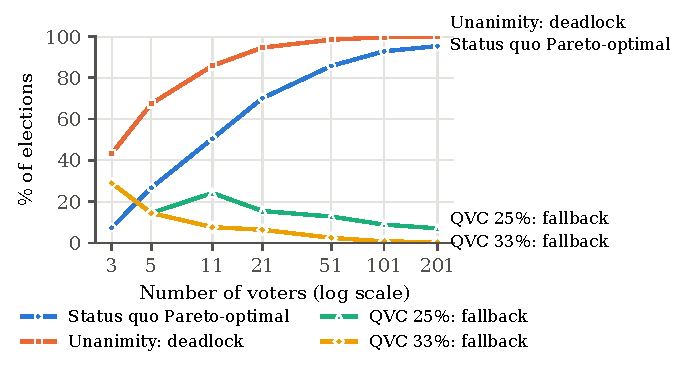
\includegraphics[width=0.85\linewidth]{fig_deadlock}
\caption{Deadlock under unanimity as the assembly grows}\label{fig:deadlock}
\figurenotes{Share of elections in which: the status quo lies in the convex hull of the voters' ideal
points, so that no option can be unanimously preferred to it (Proposition~\ref{prop:gridlock}); unanimity
with the status quo as default keeps it because no proposal is preferred to it by every voter; \QVC\ with
a blocking quota of 25\% or 33\% finds every option vetoed by the quota and falls back on the
least-vetoed options, still deciding. Spatial culture, 7 proposals and the status quo, 1,000 elections
per point. Values in Table~\ref{tab:deadlock_n}.}{Monte Carlo simulation, \texttt{experiments.py};
\texttt{figures.py}.}
\end{figure}

%% ================================================================================================
%%  4. What research says about veto rights
%%  Notes: ../literature/consensus-2026-10_review-notes.md (the Consensus review), research-agenda.md §4
%% ================================================================================================
\section{What research says about veto rights}\label{sec:veto}

The literature on veto rights is split across three traditions that rarely cite each other: committee
and legislative bargaining (economics and political science), the choice of a compromise from a finite
set of options (social choice), and the study of consensus in real organisations. We review each, then
summarise the evidence in Table~\ref{tab:evidence}.

\subsection{Unanimity against majority with a veto}

The sharpest comparison concerns committees that decide between a reform and the status quo.
\citet{BoutonLlorenteSaguerMalherbe2018} compare unanimity with \emph{majority rule with veto power}, in
which members vote by majority but each may also cast a veto that blocks the reform. When members share a common interest but hold private information, the second rule
aggregates information better and dominates unanimity in large committees: under unanimity a member
who doubts the reform can only block it, whereas majority with veto lets them vote against it without
blocking and keeps the veto for the case where they are sure. A laboratory study confirms the ranking
\citep{BoutonLlorenteSaguerMalherbe2017}. The lesson the authors draw, and the Consensus review
endorses, is to separate the right to \emph{block an unacceptable outcome} from the right to
\emph{approve a choice}.

Bargaining models and experiments point the same way. Unanimity can be uniquely inefficient, with
costly conflict and delay \citep{MiettinenVanberg2025,PiazoloVanberg2025}; laboratory committees show
delay and a larger share captured by members who hold a veto
\citep{LaingSlotznick1991,KagelSungWinter2010,AgranovTergiman2019}. The case for unanimity is
conditional: it can improve the honesty of deliberation when members are held responsible for their
votes \citep{BreitmoserValasek2024}, and the comparison with majority depends on what proposers know
\citep{GlyniaThumXefteris2026}.

\subsection{Veto players, agenda power and the status quo}

In political systems, each additional veto player, and each increase in the distance between their
positions, shrinks the set of policies that can replace the status quo; policy stability, or gridlock,
follows \citep{Tsebelis1995,Tsebelis2002}. The status quo is not a neutral fallback: the worse it is for
the others, the more an agenda setter can extract \citep{RomerRosenthal1978}, and whoever proposes holds
power that grows with the patience of the others and the voting rule \citep{BaronFerejohn1989,Harrington1990}.
When today's decision becomes tomorrow's status quo, the dynamics compound: an endogenous status quo
produces inertia and inefficiency \citep{DziudaLoeper2016,AnesiSeidmann2015}, and in laboratory
committees extra rounds strengthen the vetoer \citep{Nunnari2021}; on the stability of policies with
veto players, see \citet{AnesiDuggan2017}. A veto also
discourages experimentation, since a member who may lose from a reform can block the trial that would
reveal its value \citep{AnesiBowen2021}. The best use of a veto player is sometimes to delegate the
choice to them within an interval fixed in advance \citep{KartikKleinerVanWeelden2021}.

Two implications for our design follow. First, the status quo should not be a privileged default:
giving it that role turns every veto into a vote for inertia. Second, the agenda should not be
sequential: in sequential and amendment procedures, the order in which options are put to the vote can be
manipulated \citep{McKelvey1976,BarberaGerber2017}. Under H2, voters judge all options at once, which
removes the agenda setter's power, provided the rule is robust to the composition of the agenda
(Section~\ref{sec:aggregation}).

\subsection{How many rounds?}

There is no general result that more rounds are better. In proposal models with single-peaked
preferences, recent procedures reach the Condorcet winner in one round, where each voter either proposes
or votes \citep{Gersbach2025propose}, or in two rounds with randomly drawn proposers
\citep{GersbachValkanova2024}; see also \citet{Gersbach2024forms}. When voting is costly, a sequence of
rounds with a falling threshold can be optimal \citep{Bognar2015}. In bargaining with vetoes and an
endogenous status quo, however, extra rounds tend to create delay and to strengthen vetoers rather than
improve decisions \citep{Nunnari2021,DziudaLoeper2016}. The Consensus review concludes that one or two
rounds suffice in structured settings, and that robustness of fast procedures to hard vetoes is an open
question. Our design uses one ballot round, with at most one revision round (Section~\ref{sec:safeguards}).

\subsection{Compromise rules with vetoes}

Social choice offers several procedures that select a compromise from a finite set of options by
vetoing.
\begin{itemize}
  \item \textbf{Voting by veto} \citep{Mueller1978}: each of $n$ members proposes one option, the status
  quo is added, and in a random order each member strikes one option; the last one standing wins. The
  procedure always decides and no member gets their worst outcome, but it is not anonymous and needs
  exactly one more option than voters.
  \item \textbf{Proportional veto} \citep{Moulin1981,Moulin1982,Moulin1983}: coalitions veto a share of
  the options equal to their share of the voters (Definition~\ref{def:pvc}). The core is never empty,
  and procedures of successive vetoes can implement it in strong equilibrium. The core can be computed,
  and an option selected from it by an anonymous and neutral rule, in polynomial time
  \citep{IanovskiKondratev2021}; \citet{KondratevIanovski2024} study which rules that always select from
  the core are monotonic, satisfy participation or ignore options that everyone ranks last.
  \item \textbf{Fallback bargaining} \citep{BramsKilgour2001}: members descend their rankings in
  lockstep until an option appears on every list. The outcome is Pareto-optimal and maximises the worst
  rank, but it may miss the Condorcet winner and even a majority's first choice; with an ``impasse'' line,
  below which members refuse to go, it can end in no agreement.
  \item \textbf{Majoritarian compromise} \citep{SertelYilmaz1999,HurwiczSertel1999}: the same descent,
  stopped at the first depth at which an option appears in the lists of a majority; it is
  majoritarian-optimal and implementable in subgame-perfect equilibrium.
  \item \textbf{Shortlisting and veto-rank} for two parties: one party shortlists, the other chooses
  \citep{BarberaCoelho2017,BarberaCoelho2022}; or parties strike options alternately
  \citep{Anbarci1993}, or in proportion to ranks \citep{LaslierNunezSanver2021}. These rules can have
  several equilibria, some Pareto-inefficient, and \citet{CaillouxNapolitanoSanver2022} argue that several
  ``compromise'' rules fail to select an outcome that is a compromise once the result is known.
\end{itemize}
None of these was designed for an open agenda. Section~\ref{sec:aggregation} shows that fallback
bargaining, the majoritarian compromise, sequential vetoes and the proportional veto core all reward
flooding the agenda with clones.

\subsection{Consensus in practice}

Organisations that decide ``by consensus'' rarely give every member a hard veto. The Internet
Engineering Task Force works by \emph{rough consensus}: lack of disagreement matters more than agreement,
and consensus is reached when all objections have been addressed, though not necessarily accommodated;
an objection judged unpersuasive does not block \citep[\S\S2--3]{Resnick2014rfc7282}. In bodies that
decide by tacit consent, the formal right of every member to object is constrained by social pressure
and by the prospect of a fallback majority vote, so that effective veto power is much smaller than the
rule suggests \citep{Krick2017}. Where a hard individual veto has been taken literally, as in the
\emph{liberum veto} of the Polish--Lithuanian Sejm, it paralysed decision-making \citep{Rohac2008}.
Formal institutions grant vetoes to coalitions instead: the Council of the European Union's blocking
minority needs at least four members \citep{TEU2016art16}.

The closest existing procedure to the one we recommend is the Debian constitution
\citep[\S A.5]{Debian2024constitution}. Developers rank all the options of a general resolution,
including the default option ``None of the above''; options ranked above the default are deemed
acceptable. An option is dropped if too few voters rank it above the default (a quorum) or if it fails
to beat the default by its required majority (3:1 for constitutional amendments); the winner among the
remaining options is chosen by the Schulze method. Debian thus combines open amendments, full ranked
ballots, an acceptability line and a clone-independent Condorcet method, but it keeps the default
option as a privileged fallback, a choice that suits a project in which ``no change'' is a safe
outcome.

\begin{table}[htbp]\centering\small
\caption{What the literature supports}\label{tab:evidence}
\begin{tabularx}{\linewidth}{>{\raggedright\arraybackslash}X l >{\raggedright\arraybackslash}p{0.33\linewidth}}
\toprule
Claim & Evidence & Main sources \\
\midrule
Full unanimity is rarely optimal for open choices: it raises delay, status-quo bias and holdout power
  & Strong & \citet{Tsebelis2002,DziudaLoeper2016,MiettinenVanberg2025,KagelSungWinter2010}; Prop.~\ref{prop:gridlock} \\
Majority with a separate veto beats unanimity for information aggregation
  & Strong & \citet{BoutonLlorenteSaguerMalherbe2018,BoutonLlorenteSaguerMalherbe2017} \\
No rule is strategy-proof; the majority principle and minority vetoes conflict
  & Theorem & \citet{Gibbard1973,Satterthwaite1975}; Prop.~\ref{prop:majority-veto} \\
Simultaneous voting on all options removes agenda-setter power; clone independence removes the gain
  from flooding & Strong (theory) & \citet{McKelvey1976,Tideman1987,Schulze2011} \\
Condorcet winners exist in most structured electorates
  & Strong & \citet{RegenwetterEtAl2006,TidemanPlassmann2012}; Table~\ref{tab:cw_probability} \\
Fallback, shortlisting and veto-rank rules are useful second-best compromise devices
  & Moderate & \citet{BramsKilgour2001,BarberaCoelho2022,CaillouxNapolitanoSanver2022} \\
One or two rounds suffice in structured proposal settings
  & Moderate & \citet{GersbachValkanova2024,Gersbach2025propose} \\
In practice, a formal individual veto is socially constrained
  & Weak to moderate & \citet{Krick2017,Resnick2014rfc7282} \\
\bottomrule
\end{tabularx}
\figurenotes{Evidence: strong, several formal results and experiments or field evidence agree;
moderate, formal results under restrictive assumptions; weak, case studies. Adapted and extended from
the Consensus review of October 2026 (its Figure~6).}{Sections~\ref{sec:limits}--\ref{sec:aggregation}
of this note.}
\end{table}

%% ================================================================================================
%%  5. Aggregating full ballots on an open agenda
%%  Notes: research-agenda.md §5; code: simulations/python/voting.py (rules), examples.py (E2)
%% ================================================================================================
\section{Aggregating full ballots on an open agenda}\label{sec:aggregation}

Under H2 every voter ranks every option, so the procedure needs a rule that aggregates full rankings. This
section compares the main families of rules on the properties that matter under H1--H3.

\subsection{The families of rules}

\begin{itemize}
  \item \textbf{Positional rules} give points by rank: plurality (one point to the first choice), Borda
  ($m-k$ points to the $k$-th choice; \citealp{Young1974}).
  \item \textbf{Runoff rules}: instant-runoff voting (IRV) eliminates the option with the fewest first
  choices until one has a majority.
  \item \textbf{Condorcet methods} elect the Condorcet winner when there is one and differ in how they
  resolve cycles. Copeland counts pairwise wins; Minimax (Simpson--Kramer) minimises the worst pairwise
  defeat \citep{Simpson1969}; Kemeny--Young finds the ranking that disagrees least with the voters'
  pairwise preferences \citep{Kemeny1959,YoungLevenglick1978}; Ranked Pairs locks pairwise majorities
  from the strongest down, skipping any that would close a cycle \citep{Tideman1987}; the Schulze method
  elects the option whose strongest chains of pairwise victories against every other option are at
  least as strong as the reverse chains \citep{Schulze2011}; Split Cycle discards the weakest majority in
  every cycle and elects the options left undefeated \citep{HollidayPacuit2023splitcycle}, and Stable
  Voting refines it to a single winner \citep{HollidayPacuit2023stable}.
  \item \textbf{Evaluative rules} ask for grades rather than rankings: approval voting elects the option
  the most voters find acceptable \citep{BramsFishburn1978,LaslierSanver2010}; Majority Judgment elects
  the option with the best median grade \citep{BalinskiLaraki2007,BalinskiLaraki2011}; see
  \citet{FelsenthalMachover2008} for a critical evaluation.
  \item \textbf{Probabilistic rules}: maximal lotteries choose a lottery over options that no other
  lottery beats in expected pairwise majority \citep{Fishburn1984,LaffondLaslierLeBreton1993}; they are
  the only rule with a set of strong consistency properties \citep{BrandlBrandtSeedig2016}, but a group
  choosing a single option by lot is a hard sell for most organisations.
  \item \textbf{Compromise rules} with vetoes, reviewed in Section~\ref{sec:veto}: fallback bargaining,
  the majoritarian compromise, voting by veto and the proportional veto core.
\end{itemize}
Kemeny--Young and Dodgson's rule are NP-hard to compute \citep{BartholdiToveyTrick1989hard}; all the
other rules above run in polynomial time, Schulze in $O(m^3)$ after the $O(nm^2)$ count of pairwise
preferences. \citet{ElkindFaliszewskiSlinko2015} show that many of these rules can be read as finding the
nearest ``consensus'' profile (unanimous, or with a Condorcet winner) under some distance between
profiles, which makes the choice of a rule a choice of what counts as consensus. \citet{BrandtEtAl2016handbook}
survey the axiomatic and computational results on all these rules.

\begin{table}[htbp]\centering\small
\caption{Properties of the rules compared}\label{tab:properties}
\footnotesize
\begin{tabular}{l c c c c c c}
\toprule
Rule & \shortstack{Condorcet\\winner} & \shortstack{Independent\\of clones} & Monotonic & Polynomial & \shortstack{Uses\\vetoes} & \shortstack{Never\\stuck} \\
\midrule
Plurality              & $\times$     & $\times$     & \checkmark & \checkmark & $\times$   & \checkmark \\
IRV                    & $\times$     & \checkmark   & $\times$   & \checkmark & $\times$   & \checkmark \\
Borda                  & $\times$     & $\times$     & \checkmark & \checkmark & $\times$   & \checkmark \\
Copeland               & \checkmark   & $\times$     & \checkmark & \checkmark & $\times$   & \checkmark \\
Minimax                & \checkmark   & $\times$     & \checkmark & \checkmark & $\times$   & \checkmark \\
Kemeny--Young          & \checkmark   & $\times$     & \checkmark & $\times$   & $\times$   & \checkmark \\
Ranked Pairs           & \checkmark   & \checkmark   & \checkmark & \checkmark & $\times$   & \checkmark \\
Schulze                & \checkmark   & \checkmark   & \checkmark & \checkmark & $\times$   & \checkmark \\
Split Cycle$^a$        & \checkmark   & \checkmark   & \checkmark & \checkmark & $\times$   & \checkmark \\
\midrule
Approval               & $\times$     & \checkmark$^b$ & \checkmark & \checkmark & \checkmark$^c$ & \checkmark \\
Majority Judgment      & $\times$     & \checkmark$^b$ & \checkmark & \checkmark & \checkmark$^c$ & \checkmark \\
\midrule
Fallback bargaining    & $\times$     & $\times$     & \checkmark & \checkmark & $\times$   & \checkmark \\
\quad with impasse     & $\times$     & $\times$     & \checkmark & \checkmark & \checkmark & $\times$   \\
Majoritarian compromise & $\times$    & $\times$     & \checkmark & \checkmark & $\times$   & \checkmark \\
Unanimity, status quo default & $\times$ & \checkmark & \checkmark & \checkmark & \checkmark & $\times$ \\
Schulze within the PVC & $\times$ & $\times$ & --- & \checkmark & \checkmark$^d$ & \checkmark \\
\QVC($\theta$), Section~\ref{sec:procedure} & $\times^e$ & \checkmark & \checkmark$^f$ & \checkmark & \checkmark & \checkmark \\
\bottomrule
\end{tabular}
\figurenotes{Condorcet winner: elects it whenever it exists. Independent of clones: Definition~\ref{def:clones}.
Monotonic: raising the winner in some rankings never makes it lose. Never stuck: always selects an option
in a fixed number of rounds without a privileged default (Definition~\ref{def:decisive}). $\times$: fails
in some profiles; ---: not established, to our knowledge. $^a$Not resolute: ties are frequent and need a
tie-break. $^b$When voters grade or approve clones alike. $^c$The lowest grade, or non-approval, acts as a
veto mark but blocks nothing. $^d$PVC: proportional veto core; veto power read from the bottom of the rankings. $^e$Elects the Condorcet
winner of the admissible options (Proposition~\ref{prop:condorcet-admissible}). $^f$For changes in the
rankings that leave the veto marks unchanged.}{\citet{Tideman1987,Schulze2011,HollidayPacuit2023splitcycle,
BramsKilgour2001,Felsenthal2012review,BartholdiToveyTrick1989hard}; Propositions~\ref{prop:pvc-clones}
and~\ref{prop:decisive}--\ref{prop:qvc-clones}; simulations of Table~\ref{tab:clones}.}
\end{table}

Table~\ref{tab:properties} summarises the properties; \citet{Felsenthal2012review} reviews the paradoxes
that afflict each rule in more detail. Three properties sort the candidates for our use.

\subsection{An open agenda calls for independence of clones}\label{sec:clones}

When anyone can propose options, the composition of the agenda becomes a strategy. Adding variants of an
option, its clones, affects rules in three ways \citep{Tideman1987}: under plurality the clones split
their supporters' votes and lose (vote splitting); under Borda's rule they push other options down
everyone's ranking and gain (teaming); under some other rules they can crowd out third options. A
faction can therefore flood the agenda with variants of its favourite, or, under plurality, sink an
option by proposing its near-copies. Ranked Pairs, the Schulze method and Split Cycle are independent of
clones \citep{Tideman1987,ZavistTideman1989,Schulze2011,HollidayPacuit2023splitcycle}; Copeland, Minimax
and Kemeny--Young are not.

Veto-based compromise rules are exposed too, because the number of options enters their definition. In
fallback bargaining, clones of the majority's favourite fill the top of the majority's rankings and delay
the depth at which the compromise appears on every list. In the proportional veto core, a coalition's
veto power is a share of the number of options, so each clone added by the majority costs the minority a
veto that it can no longer spend elsewhere.

\begin{proposition}[Flooding defeats proportional veto]\label{prop:pvc-clones}
Neither the proportional veto core nor fallback bargaining is independent of clones: there are profiles
in which adding clones of an option outside the core (respectively, not chosen) brings that option into
the core (respectively, gets it chosen).
\end{proposition}

Example~E2 of Section~\ref{sec:examples} gives such a profile: in Example~E1, the 49\% minority blocks the
majority's favourite $A$, which is outside the core; once the majority proposes two variants of $A$, the
minority's three vetoes no longer cover them all, $A$ enters the core, and Schulze within the core elects
$A$ (Table~\ref{tab:examples}). In our simulations, three clones of a losing option change the winner of
the proportional veto core with Schulze in 15\% of polarised elections and in 54\% under the impartial
culture; they change the outcome of fallback bargaining in 25--36\% of elections, of the majoritarian
compromise in 23--52\% and of Borda's rule in 14--24\%, but never that of Schulze, Ranked Pairs or Split
Cycle (Table~\ref{tab:clones}).

Independence of clones also answers the agenda-setting concern of Section~\ref{sec:veto}. With all
options on one ballot, nobody controls the order of votes; with a clone-independent rule, nobody gains
by inflating the agenda. H1 and H2 together then neutralise most of the power that proposal rights confer
in sequential procedures \citep{BaronFerejohn1989,BarberaGerber2017}.

\subsection{Majority efficiency, manipulation and welfare}

Condorcet methods are the natural candidates when the group wants the majority principle respected
whenever it can be. Among them, Ranked Pairs and Schulze are Condorcet- and Smith-consistent, independent
of clones, monotonic and computable for any realistic number of options. Schulze is used by many organisations, Debian among them
\citep{Debian2024constitution}; Split Cycle adds stronger protections against spoilers and no-show effects at the cost of
frequent ties \citep{HollidayPacuit2023splitcycle}.

On manipulation, \citet{GreenArmytageTidemanCosman2016} compare 54 rules on survey data, spatial models
and random cultures: IRV and its Condorcet hybrid (elect the Condorcet winner, else run IRV) are the
least manipulable, while most rules have very similar utilitarian efficiency, with plurality,
anti-plurality and random dictatorship clearly worse. Adding a Condorcet step to a rule almost never
creates new opportunities for manipulation. Plurality is the rule experts like least \citep{Laslier2012loser}.
Section~\ref{sec:simulation} repeats such a comparison for our setting, with vetoes and an open agenda.

%% ================================================================================================
%%  6. The procedure: Condorcet with a blocking quota
%%  Notes: research-agenda.md §6; proofs in A_proofs.tex; algorithms in B_algorithms.tex
%%  Code: simulations/python/voting.py (qvc, --check), examples.py (table examples, --check)
%% ================================================================================================
\section{The procedure: Condorcet with a blocking quota}\label{sec:procedure}

\subsection{Design principles}

Sections~\ref{sec:limits}--\ref{sec:aggregation} translate into six principles.
\begin{enumerate}[label=P\arabic*]
  \item \textbf{One simultaneous ballot on the whole agenda.} Voters judge all options at once (H2): no
  sequential or amendment agenda, hence no power for whoever orders the votes (Section~\ref{sec:veto}).
  \item \textbf{Ranking and blocking are separate acts.} The ballot has a ranking and an acceptability
  line; only the line is a veto. This is the separation the literature favours
  \citep{BoutonLlorenteSaguerMalherbe2018}.
  \item \textbf{Vetoes are held by coalitions, not individuals.} An option is excluded only if a blocking
  minority, a share $\theta$ of the voters, finds it unacceptable: minority protection without holdouts
  (Propositions~\ref{prop:majority-veto} and~\ref{prop:gridlock}).
  \item \textbf{The status quo is an option like the others.} It can be ranked, vetoed and elected, but
  it is never the default: vetoes cannot become a vote for inertia.
  \item \textbf{The aggregation is clone-independent.} The open agenda (H1) must not reward flooding
  (Section~\ref{sec:clones}).
  \item \textbf{A decision is guaranteed.} If every option is vetoed by a blocking minority, the
  least-vetoed options are kept rather than none (R2).
\end{enumerate}

\subsection{The procedure}

\begin{definition}[Admissible options; $\theta$-compromise]\label{def:compromise}
Let $0 < \theta \le 1/2$. The \emph{admissible} options are
$\Adm = \{x \in \Opts : \veto(x) < \theta n\}$ if this set is not empty, and the least-vetoed options
$\arg\min_x \veto(x)$ otherwise. The \emph{$\theta$-compromise} is the Condorcet winner of $\Adm$, when it
exists.
\end{definition}

The definition is lexicographic: first, the outcome must be acceptable to all but a minority smaller than
$\theta$, if any option is; second, among such options, the majority decides. It is our reading of R1.
When the Condorcet winner of the whole agenda is acceptable to all but such a minority, it is the
$\theta$-compromise; when a blocking minority finds it unacceptable, as in Example~E1, the compromise is
the best option, in the majority sense, that the minority can live with.

\begin{algorithm}[htbp]
\caption{\QVC($\theta$): Condorcet with a blocking quota}\label{alg:qvc}
\begin{algorithmic}[1]
\Require options $\Opts$ (all proposals and the status quo), ballots $(\wpref_i, V_i)_{i \in \Voters}$,
  quota $\theta \in (0, 1/2]$, an order of the options drawn at random before the vote (for exact ties)
\State $\veto(x) \gets |\{i : x \in V_i\}|$ for every $x \in \Opts$ \Comment{veto counts}
\State $\Adm \gets \{x : \veto(x) < \theta n\}$
\If{$\Adm = \emptyset$} $\Adm \gets \arg\min_x \veto(x)$ \Comment{fallback: never empty}
\EndIf
\State $\Maj(x,y) \gets |\{i : x \pref_i y\}|$ for $x, y \in \Adm$ \Comment{pairwise counts}
\State $W \gets$ Schulze winners of $\Adm$ \Comment{Appendix~\ref{app:algorithms}}
\If{$|W| > 1$} $W \gets \arg\min_{x \in W} \veto(x)$, then the Schulze winners of $W$, then the first
  in the random order
\EndIf
\State \Return the option in $W$; publish $\veto$, $\Adm$ and the matrix $\Maj$
\end{algorithmic}
\end{algorithm}

Algorithm~\ref{alg:qvc} computes the $\theta$-compromise when it exists and completes it with the
Schulze method otherwise. Ranked Pairs could replace Schulze without changing any of the properties below.
The computation takes $O(nm^2 + m^3)$ operations, a fraction of a second for hundreds of options.

\subsection{Properties}

\begin{proposition}[Decisive, with no default advantage]\label{prop:decisive}
\QVC($\theta$) selects exactly one option, in one ballot round, for every profile. It treats every option,
the status quo included, in the same way, and its outcome does not depend on the order in which the
options were proposed (except through the random order that breaks exact ties).
\end{proposition}

\begin{proposition}[Acceptability guarantee]\label{prop:acceptability}
If some option is vetoed by fewer than $\theta n$ voters, so is the winner of \QVC($\theta$): more than a
share $1-\theta$ of the voters find it acceptable. Otherwise the winner is among the least-vetoed
options. Hence the winner is vetoed by at least $\theta n$ voters only if every option is, and no rule
has a lower probability of electing an option vetoed by a blocking minority.
\end{proposition}

\begin{proposition}[Majority within the admissible options]\label{prop:condorcet-admissible}
The winner of \QVC($\theta$) is in the Smith set of $\Adm$ and is not Pareto-dominated. If $\Adm$ has a
Condorcet winner, it wins; in particular the Condorcet winner of the whole agenda wins whenever fewer
than $\theta n$ voters veto it.
\end{proposition}

\begin{proposition}[Independence of clones]\label{prop:qvc-clones}
\QVC($\theta$) is independent of clones (Definition~\ref{def:clones}), up to the random order that breaks
exact ties.
\end{proposition}

The proofs are in Appendix~\ref{app:proofs}; the code checks Propositions~\ref{prop:decisive}--\ref{prop:qvc-clones} on random profiles
(Appendix~\ref{app:simulation}). The guarantees have a price, which is the subject of the
last result.

\begin{proposition}[Strategic blocking]\label{prop:blocking}
Under \QVC($\theta$), any coalition of at least $\theta n$ voters can make any option inadmissible by
vetoing it, which defeats that option whenever another option stays admissible. If $\theta \le (m-1)/m$,
and in particular for every $\theta \le 1/2$, there are profiles in which, whatever the winner $w$, at
least $\theta n$ voters prefer some other option to $w$, and can thus block $w$ by vetoing it although
they find it acceptable.
\end{proposition}

Proposition~\ref{prop:blocking} is the strategic face of Proposition~\ref{prop:majority-veto}: the power to
block an unacceptable option is also the power to block an acceptable one. \citet{Greenberg1979} gives
the general threshold: an option that no coalition of size $\theta n$ wants to replace exists for every
profile only if $\theta > (m-1)/m$, or $\theta > d/(d+1)$ in $d$ dimensions, that is, only if the veto is
weaker than majority rule. A sincere veto is cheap to cast and a strategic one is no dearer, so
safeguards must come from the procedure around the vote (Section~\ref{sec:safeguards}). The proportional
veto core avoids the problem, since it is defined as the set of options no coalition can block given its
proportional veto power \citep{Moulin1981,Moulin1982}, but it fails independence of clones
(Proposition~\ref{prop:pvc-clones}), which H1 makes essential.

\subsection{Worked examples}\label{sec:examples}

Table~\ref{tab:examples} applies nine rules to four small profiles.

% Generated by simulations/python/examples.py -- do not edit by hand
\begin{table}[htbp]\centering\footnotesize
\setlength{\tabcolsep}{4pt}
\caption{Winners in the worked examples}\label{tab:examples}
\sbox{\tabbox}{\begin{tabular}{lrrrrrrrrr}
\toprule
Example & Plur. & Borda & Schul. & Fallb. & PVC & Unan. & Q 25\% & Q 33\% & Q 50\% \\
\midrule
E1 (compromise) & A & B & A & B & B & B & B & B & A \\
E2 (flooding) & A & A & A & A & A & B & B & B & A \\
E3 (cycle) & A & A & A & B & A & C (stuck) & B (fb) & A & A \\
E4 (status quo) & X & X & X & Y & X & S (stuck) & X & X & X \\
\bottomrule
\end{tabular}}
\usebox{\tabbox}
\tabnotes{E1: 51 voters rank A, B, C and veto C; 49 rank B, C, A and veto A. E2: E1 after the majority proposes two variants of A, ranked just below A by the majority and last by the minority, which vetoes them. E3: 35 voters rank A, B, C; 33 B, C, A; 32 C, A, B; each bloc vetoes its last option. E4: 99 voters rank X, Y, S and veto S; one voter ranks S, Y, X and vetoes X and Y. The status quo is C in E1--E3 and S in E4. Stuck: no proposal passes and the status quo stays; fb: every option is vetoed by the quota and QVC keeps the least-vetoed ones. Fallb.: fallback bargaining; PVC: Schulze within the proportional veto core; Unan.: unanimity with the status quo as default; Q $x$: QVC with a blocking quota $\theta = x$.}
{Profiles of Section~\ref{sec:examples}; \texttt{examples.py}.}
\end{table}


\begin{itemize}
  \item \textbf{E1, majority or compromise.} $A$ is the Condorcet winner (51 to 49 against both others)
  and plurality and Schulze elect it. The 49\% minority, however, ranks $A$ last and vetoes it, while $B$
  is everyone's first or second choice. Borda's rule, fallback bargaining, the proportional veto core and
  \QVC\ with $\theta \le 49\%$ elect $B$; \QVC(1/2) treats a 49\% veto as insufficient and elects $A$.
  Which answer is right is the choice of $\theta$.
  \item \textbf{E2, flooding.} The majority adds two variants of $A$. Borda's rule, fallback bargaining
  and the proportional veto core now elect $A$ (Proposition~\ref{prop:pvc-clones}); \QVC\ is unchanged,
  because each variant inherits the minority's vetoes.
  \item \textbf{E3, a cycle.} $A$ beats $B$ (67--33), $B$ beats $C$ (68--32), $C$ beats $A$ (65--35);
  Schulze breaks the weakest link and elects $A$. With $\theta = 1/4$ every option is vetoed by about a
  third of the voters, so \QVC\ falls back on the least-vetoed option, $B$; with $\theta = 1/3$, $C$ (35
  vetoes) is excluded and $A$ wins. Unanimity keeps the status quo $C$, since neither proposal is
  preferred to it by everyone.
  \item \textbf{E4, the status-quo trap.} One voter prefers the status quo to everything and vetoes both
  proposals. Unanimity keeps the status quo against 99 voters; \QVC\ elects $X$, since one veto is far
  below any blocking quota.
\end{itemize}

\subsection{Choosing the quota and the details}\label{sec:theta}

\paragraph{The quota.} $\theta$ sets the size of the smallest minority whose objection counts. The
simulations of Section~\ref{sec:simulation} (Figure~\ref{fig:theta}) show three regimes.
\begin{itemize}
  \item \emph{At 15--20\% and below}, in an assembly of a hundred voters where each voter vetoes 35--40\% of
  the options, every option is vetoed by the quota and the fallback decides in most elections: the
  procedure elects the least-vetoed option, which is approval voting on acceptability. Each individual
  veto is then only a negative vote, and the result is easily manipulated.
  \item \emph{Between 25\% and 40\%}, the veto excludes the options that a substantial minority rejects
  and the majority decides among the others; the fallback is rare.
  \item \emph{From 40\% upwards}, the veto almost never binds before majority rule would and \QVC\ is the
  Schulze method.
\end{itemize}
We recommend $\theta = 1/3$ as the default: it is the blocking third that corresponds to the two-thirds
supermajorities common in statutes, close to the 35\% blocking minority of the Council of the European
Union and to the 36\% implied by the 64\% rule of \citet{CaplinNalebuff1988}. A group that values
consensus more than majority can go down to $\theta = 1/4$; going lower brings back the problems of the
individual veto. In a small group, the quota is a number of voters, $\lceil \theta n \rceil$: with ten
voters and $\theta = 1/3$, four vetoes exclude an option. Below five voters, a quota of two vetoes keeps a
single member from blocking alone.

\paragraph{The status quo.} By default the status quo is an ordinary option (P4). Where a change is
costly or irreversible, the group may wish to protect it, as Debian does: the winner must then beat the
status quo by a stated ratio (2:1, say), failing which the status quo stays. This reintroduces inertia
on purpose and should be reserved for such decisions.

\paragraph{The ballot.} A ranking with ties allowed, plus the acceptability line. With many options,
a grade-style form is easier: each option receives one of ``excellent'', ``good'', ``fair'', ``poor'' or
``unacceptable'', voters may order options within a grade, and the ranking and the vetoes are read from
the form. Options left blank are ranked last and not vetoed. Results should publish the veto counts, the
admissible set and the pairwise matrix, so that any member can check the outcome.

\subsection{Safeguards against strategic vetoing}\label{sec:safeguards}

Proposition~\ref{prop:blocking} cannot be removed by the counting rule; it can be contained by the
procedure around it.
\begin{itemize}
  \item \textbf{Named and reasoned vetoes.} A veto is public and states a reason, as an objection must in
  the IETF's rough consensus \citep{Resnick2014rfc7282}. Responsibility for one's vote changes behaviour in
  committees \citep{BreitmoserValasek2024}, and social constraints are what keeps formal vetoes in check
  in consensus bodies \citep{Krick2017}. A chair or a panel may rule a veto without a reason void.
  \item \textbf{One revision round, only when needed.} If the fallback was used (no option acceptable
  to more than $1-\theta$ of the voters), the results are published, the nomination opens again for a
  fixed time for compromise proposals, and a second ballot is held; its result is final. Two rounds at
  most keep R2 while giving a divided group a chance to find a compromise, in line with the evidence that
  one or two rounds suffice and more rounds strengthen vetoers
  \citep{GersbachValkanova2024,Nunnari2021}.
  \item \textbf{Veto budgets across decisions, not within one.} In a body that decides repeatedly, a
  limited stock of vetoes per member and per period, which can be saved for decisions that matter more,
  discourages routine blocking \citep[on storable votes]{Casella2005}. A budget within one decision would
  break independence of clones: each clone added would cost a veto.
  \item \textbf{No lower quota than needed.} The manipulability of the procedure falls quickly as
  $\theta$ rises (Figure~\ref{fig:theta}).
\end{itemize}

%% ================================================================================================
%%  7. Simulation evidence
%%  Notes: research-agenda.md §7; details in C_simulation.tex
%%  Code: simulations/python/cultures.py, experiments.py (tables perf_*, manipulability, clones,
%%        theta_sweep), figures.py (fig_theta)
%% ================================================================================================
\section{Simulation evidence}\label{sec:simulation}

The propositions say what the procedure guarantees; they do not say how often the guarantees bite, nor
what they cost in the typical case. A Monte Carlo study answers both, and compares \QVC\ with twenty
other rules on the same elections.

\subsection{Design}

Each simulated election has 101 voters and 8 options: 7 open proposals and the status quo. The
proposals are made by voters drawn at random, near their own position, so that larger blocs propose more
and near-duplicates arise as they would under H1. Three electorates (``cultures'') are used:
\begin{itemize}
  \item \textbf{spatial}: voters' ideal points spread over a plane, preferences decreasing with distance;
  \item \textbf{polarised}: two blocs of 55\% and 45\% on either side of the plane, the case in which a
  compromise matters most;
  \item \textbf{impartial}: random independent rankings, a worst case for majority rule, reported in
  Appendix~\ref{app:simulation}.
\end{itemize}
Each voter vetoes the options beyond a personal tolerance, fixed before the proposals are known, so that
the veto reflects acceptability rather than the composition of the menu; on average a voter vetoes 35--40\% of
the options. Ballots are sincere, except in the manipulation study. Each rule is scored on:
\begin{itemize}
  \item \emph{Condorcet efficiency}: how often it elects the Condorcet winner when there is one;
  \item \emph{utility efficiency}: total utility of the winner, scaled from 0 for the average option to
  100 for the best \citep{Merrill1984};
  \item \emph{worst-off efficiency}: the same scale for the voter at the 10th percentile of utility, a
  measure of how well the least satisfied voters fare;
  \item \emph{acceptance}: the share of voters who do not veto the winner, and \emph{contested}: how often
  at least a third of the voters veto the winner;
  \item \emph{deadlock}: how often the status quo stays because nothing passes.
\end{itemize}
Details, calibration and the checks of the code are in Appendix~\ref{app:simulation}.

\subsection{Results}

% Generated by simulations/python/experiments.py -- do not edit by hand
\begin{table}[htbp]\centering\footnotesize
\setlength{\tabcolsep}{4pt}
\caption{The rules compared: polarised (55/45)}\label{tab:perf_polarised}
\sbox{\tabbox}{\begin{tabular}{l>{\raggedleft\arraybackslash}p{0.087\linewidth}>{\raggedleft\arraybackslash}p{0.087\linewidth}>{\raggedleft\arraybackslash}p{0.087\linewidth}>{\raggedleft\arraybackslash}p{0.087\linewidth}>{\raggedleft\arraybackslash}p{0.087\linewidth}>{\raggedleft\arraybackslash}p{0.087\linewidth}>{\raggedleft\arraybackslash}p{0.087\linewidth}}
\toprule
Rule & Condorcet eff. (\%) & Utility eff. (\%) & Worst-off eff. (\%) & Accepted (\%) & Contested (\%) & Deadlock (\%) & Fallback (\%) \\
\midrule
Plurality & 22.4 & 34.4 & 13.3 & 63.4 & 62.1 & 0.0 & 0.0 \\
IRV & 33.1 & 70.0 & 33.3 & 68.5 & 45.6 & 0.0 & 0.0 \\
Borda & 71.2 & 94.5 & 79.1 & 75.3 & 15.2 & 0.0 & 0.0 \\
Copeland & 100.0 & 97.2 & 85.3 & 76.7 & 9.8 & 0.0 & 0.0 \\
Minimax & 100.0 & 97.4 & 85.2 & 76.6 & 10.1 & 0.0 & 0.0 \\
Schulze & 100.0 & 97.4 & 85.2 & 76.6 & 10.1 & 0.0 & 0.0 \\
Ranked Pairs & 100.0 & 97.4 & 85.1 & 76.6 & 10.2 & 0.0 & 0.0 \\
Split Cycle & 100.0 & 97.4 & 85.2 & 76.6 & 10.1 & 0.0 & 0.0 \\
\midrule
Approval & 72.2 & 95.5 & 95.0 & 78.2 & 5.9 & 0.0 & 0.0 \\
Majority Judgment & 55.3 & 88.5 & 60.1 & 73.1 & 23.9 & 0.0 & 0.0 \\
\midrule
Fallback & 53.7 & 87.7 & 79.9 & 74.7 & 18.6 & 0.0 & 0.0 \\
Fallback (impasse) & 15.7 & 3.0 & 27.2 & 60.5 & 58.1 & 100.0 & 0.0 \\
Majoritarian compromise & 62.2 & 89.1 & 69.0 & 74.1 & 20.8 & 0.0 & 0.0 \\
Sequential veto & 38.7 & 74.1 & 64.4 & 71.6 & 30.7 & 0.0 & 0.0 \\
\midrule
Unanimity & 16.2 & 8.5 & 30.7 & 61.4 & 57.4 & 97.9 & 0.0 \\
PVC + Schulze & 90.8 & 96.2 & 86.7 & 76.6 & 10.2 & 0.0 & 0.0 \\
QVC, any veto (1/n) & 72.2 & 95.5 & 95.0 & 78.2 & 5.9 & 0.0 & 100.0 \\
QVC, 10\% & 72.4 & 95.6 & 95.0 & 78.2 & 5.9 & 0.0 & 98.6 \\
QVC, 25\% & 83.2 & 96.8 & 92.8 & 77.8 & 5.9 & 0.0 & 26.9 \\
QVC, 33\% & 94.3 & 97.7 & 88.4 & 77.1 & 5.9 & 0.0 & 5.9 \\
QVC, 50\% & 99.9 & 97.4 & 85.1 & 76.6 & 10.1 & 0.0 & 0.0 \\
\bottomrule
\end{tabular}}
\usebox{\tabbox}
\tabnotes{2,000 elections, 101 voters, 8 options of which one is the status quo. Condorcet efficiency: share of the elections with a Condorcet winner (here 97.7\%) in which the rule elects it. Utility efficiency: total utility of the winner, 0 for the average option and 100 for the best \citep{Merrill1984}. Worst-off efficiency: the same for the utility of the voter at the 10th percentile. Accepted: average share of the voters who do not veto the winner. Contested: share of the elections whose winner is vetoed by at least a third of the voters. Deadlock: the status quo stays because no proposal passes. Fallback: QVC excluded every option and kept the least vetoed. QVC, $x$: Condorcet with a blocking quota $\theta = x$ (Section~\ref{sec:procedure}). Monte Carlo standard errors are at most 1.1 points.}
{Monte Carlo simulation, cultures of \texttt{cultures.py}, rules of \texttt{voting.py}; \texttt{experiments.py}.}
\end{table}


\paragraph{Condorcet methods lead on welfare.} In both structured electorates, the Condorcet methods
(Copeland, Minimax, Schulze, Ranked Pairs, Split Cycle) reach the highest utility efficiency, 99.5 in
the spatial and 97.2--97.4 in the polarised electorate (Tables~\ref{tab:perf_polarised}
and~\ref{tab:perf_spatial}). Borda's rule and the evaluative rules (approval, Majority Judgment) come next;
plurality and instant-runoff trail far behind in the polarised case, where they elect a bloc's
favourite (utility efficiency 34 and 70). This confirms, with vetoes and an open agenda, the ranking of
\citet{Merrill1984} and \citet{GreenArmytageTidemanCosman2016}.

\paragraph{Hard vetoes deadlock.} Unanimity with the status quo as default keeps it in 98--99\% of
elections, and fallback bargaining with impasse never reaches an agreement: with 101 voters, no
proposal is acceptable to everyone. Their outcome is then the status quo, whose utility efficiency is close to that of a random option. This is Proposition~\ref{prop:gridlock} in numbers.

\paragraph{The veto quota buys protection for the worst-off.} In the polarised electorate, the Schulze
winner is vetoed by at least a third of the voters in 10.1\% of elections. \QVC(1/3) halves that, to
5.9\%, the minimum any rule can reach (Proposition~\ref{prop:acceptability}): in those 5.9\% of elections
every option is vetoed by a third. It raises worst-off efficiency from 85.2 to 88.4, and it does so with
no loss of total utility (97.7 against 97.4): the compromise it picks is better for the minority bloc
and about as good on average. The cost is in Condorcet efficiency, 94.3\%: in 5.7\% of the elections that have a Condorcet winner, the
majority's preferred option is set aside because a blocking third rejects it. With $\theta = 1/4$ the
trade goes further (worst-off efficiency 92.8, Condorcet efficiency 83.2), towards the ``least-vetoed''
outcome of approval voting. In the spatial electorate, where most options are broadly acceptable,
\QVC(1/3) and Schulze agree in 99.5\% of cases with a Condorcet winner. The proportional veto core with
Schulze moves in the same direction as \QVC\ but less (worst-off efficiency 86.7, contested 10.2\%).

% Generated by simulations/python/experiments.py -- do not edit by hand
\begin{table}[htbp]\centering\footnotesize
\setlength{\tabcolsep}{4pt}
\caption{The rules compared: spatial (2D)}\label{tab:perf_spatial}
\sbox{\tabbox}{\begin{tabular}{l>{\raggedleft\arraybackslash}p{0.087\linewidth}>{\raggedleft\arraybackslash}p{0.087\linewidth}>{\raggedleft\arraybackslash}p{0.087\linewidth}>{\raggedleft\arraybackslash}p{0.087\linewidth}>{\raggedleft\arraybackslash}p{0.087\linewidth}>{\raggedleft\arraybackslash}p{0.087\linewidth}>{\raggedleft\arraybackslash}p{0.087\linewidth}}
\toprule
Rule & Condorcet eff. (\%) & Utility eff. (\%) & Worst-off eff. (\%) & Accepted (\%) & Contested (\%) & Deadlock (\%) & Fallback (\%) \\
\midrule
Plurality & 41.5 & 73.1 & 67.0 & 76.7 & 11.7 & 0.0 & 0.0 \\
IRV & 64.9 & 92.0 & 86.3 & 80.0 & 1.9 & 0.0 & 0.0 \\
Borda & 86.3 & 98.6 & 93.8 & 81.1 & 1.3 & 0.0 & 0.0 \\
Copeland & 100.0 & 99.5 & 94.9 & 81.3 & 1.1 & 0.0 & 0.0 \\
Minimax & 100.0 & 99.5 & 95.0 & 81.3 & 1.1 & 0.0 & 0.0 \\
Schulze & 100.0 & 99.5 & 95.0 & 81.3 & 1.1 & 0.0 & 0.0 \\
Ranked Pairs & 100.0 & 99.5 & 94.9 & 81.2 & 1.1 & 0.0 & 0.0 \\
Split Cycle & 100.0 & 99.5 & 95.0 & 81.3 & 1.1 & 0.0 & 0.0 \\
\midrule
Approval & 78.2 & 97.6 & 94.8 & 81.8 & 0.9 & 0.0 & 0.0 \\
Majority Judgment & 77.7 & 97.6 & 91.6 & 80.8 & 1.1 & 0.0 & 0.0 \\
\midrule
Fallback & 61.2 & 90.4 & 86.5 & 79.7 & 4.2 & 0.0 & 0.0 \\
Fallback (impasse) & 12.1 & -2.0 & -0.6 & 61.8 & 50.8 & 100.0 & 0.0 \\
Majoritarian compromise & 76.6 & 97.1 & 92.0 & 80.8 & 1.6 & 0.0 & 0.0 \\
Sequential veto & 45.2 & 81.8 & 76.9 & 78.0 & 8.4 & 0.0 & 0.0 \\
\midrule
Unanimity & 12.1 & -0.9 & 0.3 & 62.1 & 50.6 & 99.4 & 0.0 \\
PVC + Schulze & 99.5 & 99.5 & 94.8 & 81.3 & 1.1 & 0.0 & 0.0 \\
QVC, any veto (1/n) & 78.2 & 97.6 & 94.8 & 81.8 & 0.9 & 0.0 & 100.0 \\
QVC, 10\% & 78.3 & 97.6 & 94.8 & 81.8 & 0.9 & 0.0 & 96.9 \\
QVC, 25\% & 96.1 & 99.2 & 94.9 & 81.4 & 0.9 & 0.0 & 9.2 \\
QVC, 33\% & 99.5 & 99.5 & 94.9 & 81.3 & 0.9 & 0.0 & 0.9 \\
QVC, 50\% & 100.0 & 99.5 & 95.0 & 81.3 & 1.1 & 0.0 & 0.0 \\
\bottomrule
\end{tabular}}
\usebox{\tabbox}
\tabnotes{2,000 elections, 101 voters, 8 options of which one is the status quo. Condorcet efficiency: share of the elections with a Condorcet winner (here 98.6\%) in which the rule elects it. Utility efficiency: total utility of the winner, 0 for the average option and 100 for the best \citep{Merrill1984}. Worst-off efficiency: the same for the utility of the voter at the 10th percentile. Accepted: average share of the voters who do not veto the winner. Contested: share of the elections whose winner is vetoed by at least a third of the voters. Deadlock: the status quo stays because no proposal passes. Fallback: QVC excluded every option and kept the least vetoed. QVC, $x$: Condorcet with a blocking quota $\theta = x$ (Section~\ref{sec:procedure}). Monte Carlo standard errors are at most 1.1 points.}
{Monte Carlo simulation, cultures of \texttt{cultures.py}, rules of \texttt{voting.py}; \texttt{experiments.py}.}
\end{table}


\paragraph{Only clone-independent rules resist flooding.} Adding three clones of a losing option never
changes the outcome of Schulze, Ranked Pairs, Split Cycle or \QVC\ (Table~\ref{tab:clones}). It changes
that of Borda's rule in 14--24\% of elections (teaming), of fallback bargaining in 25--36\%, of the
majoritarian compromise in 23--52\%, of sequential vetoes in 68--82\%, and of the proportional veto core
in up to 54\%. Cloning the winner defeats it under plurality in 94--100\% of elections (vote splitting).

% Generated by simulations/python/experiments.py -- do not edit by hand
\begin{table}[htbp]\centering\footnotesize
\setlength{\tabcolsep}{4pt}
\caption{Share of outcomes changed by three clones}\label{tab:clones}
\sbox{\tabbox}{\begin{tabular}{l>{\raggedleft\arraybackslash}p{0.098\linewidth}>{\raggedleft\arraybackslash}p{0.100\linewidth}>{\raggedleft\arraybackslash}p{0.100\linewidth}>{\raggedleft\arraybackslash}p{0.100\linewidth}>{\raggedleft\arraybackslash}p{0.100\linewidth}>{\raggedleft\arraybackslash}p{0.100\linewidth}}
\toprule
Rule & Spatial: loser (\%) & Spatial: winner (\%) & Polarised: loser (\%) & Polarised: winner (\%) & Impartial: loser (\%) & Impartial: winner (\%) \\
\midrule
Plurality & 0.0 & 97.6 & 0.0 & 93.7 & 0.0 & 100.0 \\
IRV & 0.3 & 0.2 & 0.2 & 0.3 & 1.2 & 1.9 \\
Borda & 14.1 & 1.2 & 24.3 & 3.1 & 21.4 & 1.4 \\
Copeland & 0.2 & 0.3 & 0.5 & 0.3 & 7.7 & 3.0 \\
Minimax & 0.0 & 1.2 & 0.0 & 1.9 & 0.0 & 2.0 \\
Schulze & 0.0 & 0.0 & 0.0 & 0.0 & 0.0 & 0.0 \\
Ranked Pairs & 0.0 & 0.0 & 0.0 & 0.0 & 0.0 & 0.0 \\
Split Cycle & 0.0 & 0.0 & 0.0 & 0.0 & 0.0 & 0.0 \\
\midrule
Approval & 0.0 & 0.0 & 0.0 & 0.0 & 0.0 & 0.2 \\
Majority Judgment & 0.0 & 0.0 & 0.0 & 0.0 & 0.0 & 0.0 \\
\midrule
Fallback & 30.7 & 0.0 & 36.4 & 0.0 & 24.6 & 0.0 \\
Fallback (impasse) & 0.0 & 0.0 & 0.0 & 0.0 & 0.0 & 0.0 \\
Majoritarian compromise & 23.1 & 12.8 & 34.1 & 28.2 & 51.9 & 14.9 \\
Sequential veto & 67.8 & 0.0 & 68.7 & 0.0 & 81.9 & 0.0 \\
\midrule
Unanimity & 0.0 & 0.0 & 0.0 & 0.0 & 0.0 & 0.0 \\
PVC + Schulze & 1.2 & 0.0 & 15.1 & 0.1 & 53.9 & 4.5 \\
QVC, any veto (1/n) & 0.0 & 0.0 & 0.0 & 0.0 & 0.0 & 0.0 \\
QVC, 10\% & 0.0 & 0.0 & 0.0 & 0.0 & 0.0 & 0.0 \\
QVC, 25\% & 0.0 & 0.0 & 0.0 & 0.0 & 0.0 & 0.0 \\
QVC, 33\% & 0.0 & 0.0 & 0.0 & 0.0 & 0.0 & 0.0 \\
QVC, 50\% & 0.0 & 0.0 & 0.0 & 0.0 & 0.0 & 0.0 \\
\bottomrule
\end{tabular}}
\usebox{\tabbox}
\tabnotes{1,000 elections per culture, 101 voters, 8 options. Loser: three clones of a losing option, drawn at random, are added (teaming, or flooding the agenda); winner: three clones of the winner are added (vote splitting). A clone is a variant that every voter ranks next to the original, and grades and vetoes as the original \citep{Tideman1987}. The outcome is unchanged if the winner is the same or a clone of it. Monte Carlo standard errors at most 1.6 points.}
{Monte Carlo simulation, cultures of \texttt{cultures.py}, rules of \texttt{voting.py}; \texttt{experiments.py}.}
\end{table}


\paragraph{Vetoes are a strategic instrument.} Table~\ref{tab:manipulability} reports how often a
coalition of voters who prefer some option $y$ to the winner can elect $y$ with simple joint strategies:
ranking $y$ first and the winner last, and vetoing the winner or every option but $y$. With full coalitions, most decisive rules are manipulable in a majority of elections, as the
Gibbard--Satterthwaite theorem leads one to expect (instant-runoff is the least exposed, as in
\citealp{GreenArmytageTidemanCosman2016}); \QVC\ with $\theta < 1/2$ in nearly all, because the voters who prefer $y$ to the
winner usually number more than $\theta n$ and can veto the winner (Proposition~\ref{prop:blocking}).
The more realistic case is a small coalition, at most 10\% of the voters. Schulze, Ranked Pairs, Split Cycle and Minimax are then manipulable in only 4--7\% of structured
elections (Copeland in 20--31\%), against 37--45\% for instant-runoff and 69--85\% for
approval voting and Majority Judgment. \QVC(1/3) stands between, at 11\% in the spatial and 27\% in the
polarised electorate; \QVC(1/4) at 52--57\%. Under the impartial culture all rules are highly
manipulable. Unanimity is almost never manipulable, for the wrong reason: it rarely decides anything.

% Generated by simulations/python/experiments.py -- do not edit by hand
\begin{table}[htbp]\centering\footnotesize
\setlength{\tabcolsep}{4pt}
\caption{Share of elections a coalition can manipulate}\label{tab:manipulability}
\sbox{\tabbox}{\begin{tabular}{l>{\raggedleft\arraybackslash}p{0.089\linewidth}>{\raggedleft\arraybackslash}p{0.089\linewidth}>{\raggedleft\arraybackslash}p{0.100\linewidth}>{\raggedleft\arraybackslash}p{0.100\linewidth}>{\raggedleft\arraybackslash}p{0.100\linewidth}>{\raggedleft\arraybackslash}p{0.100\linewidth}}
\toprule
Rule & Spatial: all (\%) & Spatial: 10\% (\%) & Polarised: all (\%) & Polarised: 10\% (\%) & Impartial: all (\%) & Impartial: 10\% (\%) \\
\midrule
Plurality & 94.2 & 53.8 & 98.6 & 45.0 & 100.0 & 98.0 \\
IRV & 47.8 & 36.6 & 76.2 & 44.6 & 53.4 & 51.6 \\
Borda & 97.8 & 79.0 & 96.8 & 81.6 & 100.0 & 95.2 \\
Copeland & 96.2 & 19.8 & 96.8 & 31.2 & 100.0 & 88.4 \\
Minimax & 63.2 & 4.8 & 53.8 & 7.0 & 100.0 & 70.8 \\
Schulze & 63.2 & 4.8 & 53.8 & 6.8 & 100.0 & 71.2 \\
Ranked Pairs & 71.6 & 4.4 & 69.8 & 6.2 & 100.0 & 64.8 \\
Split Cycle & 73.0 & 5.0 & 72.2 & 7.2 & 100.0 & 72.2 \\
\midrule
Approval & 99.6 & 84.6 & 100.0 & 68.8 & 100.0 & 90.6 \\
Majority Judgment & 98.8 & 79.0 & 99.4 & 79.8 & 100.0 & 86.6 \\
\midrule
Fallback & 83.6 & 97.4 & 86.2 & 98.8 & 100.0 & 90.6 \\
Fallback (impasse) & 5.8 & 0.0 & 15.8 & 0.0 & 0.0 & 0.0 \\
Majoritarian compromise & 77.2 & 33.0 & 81.2 & 39.4 & 100.0 & 81.6 \\
Sequential veto & 76.8 & 76.8 & 63.2 & 63.2 & 69.2 & 69.2 \\
\midrule
Unanimity & 0.0 & 0.0 & 0.8 & 0.8 & 0.0 & 0.0 \\
PVC + Schulze & 98.4 & 5.8 & 87.6 & 7.0 & 100.0 & 95.4 \\
QVC, any veto (1/n) & 99.6 & 84.6 & 100.0 & 68.8 & 100.0 & 90.6 \\
QVC, 10\% & 99.6 & 84.6 & 100.0 & 68.8 & 100.0 & 90.6 \\
QVC, 25\% & 99.6 & 51.8 & 100.0 & 56.8 & 100.0 & 90.6 \\
QVC, 33\% & 99.4 & 11.0 & 100.0 & 26.6 & 100.0 & 81.8 \\
QVC, 50\% & 72.2 & 4.8 & 83.6 & 7.0 & 100.0 & 71.2 \\
\bottomrule
\end{tabular}}
\usebox{\tabbox}
\tabnotes{500 elections per culture, 101 voters, 8 options. An election counts as manipulable if, for some option $y$, voters who prefer $y$ to the winner can elect $y$ by one of three joint strategies: rank $y$ first and the winner last, vetoing the winner; the same, vetoing every option but $y$; or rank the winner last and veto it. All: every voter who prefers $y$ to the winner joins; 10\%: at most 10 of them. Other strategies may succeed where these fail: the shares are lower bounds. Monte Carlo standard errors at most 2.2 points.}
{Monte Carlo simulation, cultures of \texttt{cultures.py}, rules of \texttt{voting.py}; \texttt{experiments.py}.}
\end{table}


\paragraph{The trade-off in the quota.} Figure~\ref{fig:theta} traces the measures as $\theta$ varies.
Condorcet efficiency rises and worst-off efficiency falls with $\theta$; the fallback, frequent below
20\%, all but disappears above 30\%; small-coalition manipulability falls steeply between 20\% and 40\%.
At $\theta = 1/3$ the fallback is rare (1\% of spatial and 6\% of polarised elections), Condorcet
efficiency is at least 94\% and most of the gain in worst-off efficiency is kept; a quarter buys more protection at the price of a fallback in a quarter of polarised elections and two
to four times the small-coalition manipulability.

\begin{figure}[htbp]\centering
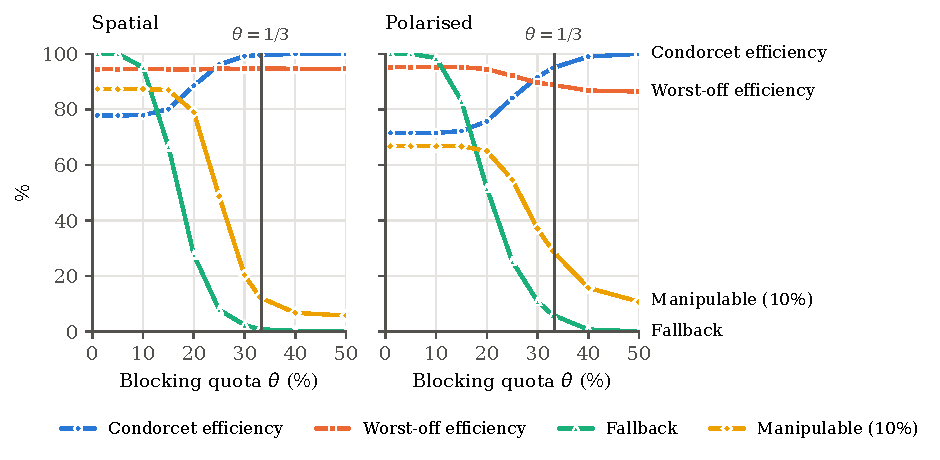
\includegraphics[width=\linewidth]{fig_theta}
\caption{QVC: what the blocking quota buys and costs}\label{fig:theta}
\figurenotes{Each line is a measure of the winner of \QVC($\theta$) as the blocking quota $\theta$
varies, from a single veto ($1/n$, plotted at 1\%) to half of the voters. Condorcet efficiency,
worst-off efficiency and fallback as in Table~\ref{tab:perf_polarised}; manipulable (10\%): share of
elections a coalition of at most 10\% of the voters can manipulate (Table~\ref{tab:manipulability}).
1,000 elections per culture (300 for manipulability), 101 voters, 8 options. The vertical line marks the
recommended quota, $\theta = 1/3$. Values in Table~\ref{tab:theta_sweep}.}{Monte Carlo simulation,
\texttt{experiments.py}; \texttt{figures.py}.}
\end{figure}

\subsection{What the simulation does not show}

The cultures are stylised: two dimensions, Euclidean preferences, a fixed tolerance for vetoes, and a
proposal process with no deliberation. The manipulation study gives full information to the coalition
and only counts three strategies, so it bounds manipulability from below; it does not model the
safeguards of Section~\ref{sec:safeguards}, which act on the willingness to veto strategically rather
than on the counting rule. Ballots from real assemblies, for instance from the PrefLib library
\citep{MatteiWalsh2013}, would test the conclusions on observed preferences; Debian's published ballots
would be a natural start.

%% ================================================================================================
%%  8. Discussion
%%  Notes: research-agenda.md §8 (open questions), author-tasks.md
%% ================================================================================================
\section{Discussion}\label{sec:discussion}

\subsection{How firm are the conclusions?}

Three conclusions rest on theorems and are not in doubt: no procedure is immune to manipulation; the
majority principle and a minority veto conflict in some profiles; and individual vetoes with the status
quo as default deadlock a large assembly. Two rest on a broad and consistent literature: Condorcet methods
achieve the best welfare among common rules when preferences have structure, and an open agenda calls for
independence of clones. The recommendation of a blocking quota of one third is a judgement on a
trade-off, supported by simulations on stylised electorates; the shape of the trade-off is robust across
our cultures, the precise numbers are not.

\subsection{Limits of this note}

The note considers a single decision. Repeated decisions raise questions it does not treat: today's
outcome becomes tomorrow's status quo \citep{DziudaLoeper2016}, vetoes can be traded or saved
\citep{Casella2005}, and reputations form. It takes preferences and proposals as given, whereas
deliberation changes both, and the IETF's practice suggests that much of the value of a consensus process
lies in how objections are discussed rather than counted \citep{Resnick2014rfc7282}. All voters have equal
weight; weighted assemblies (shareholders, federations) would need weighted counts and a weighted quota,
which the procedure accommodates but we have not analysed. Finally, the literature search behind the
Consensus review, and our own additions, focus on economics, political science and computational social
choice; work in management science on group decision support, and in law on supermajority requirements,
is not covered.

\subsection{Open questions}

\begin{itemize}
  \item \textbf{A clone-proof proportional veto?} The proportional veto core protects minorities in a
  way that no coalition can undo, but fails independence of clones; the blocking quota is clone-proof
  but open to strategic blocking (Propositions~\ref{prop:pvc-clones} and~\ref{prop:blocking}). Whether
  some rule combines independence of clones, veto power proportional to size and a non-empty core, or
  whether the three are incompatible, is open as far as we know.
  \item \textbf{Fast procedures with hard vetoes.} One- and two-round proposal procedures reach the
  Condorcet winner quickly under single-peaked preferences \citep{Gersbach2025propose,GersbachValkanova2024};
  their behaviour with binding vetoes and several dimensions is unknown (a gap also noted by the Consensus
  review).
  \item \textbf{Strategic comparison of compromise rules.} Fallback bargaining, shortlisting, veto-rank and
  proportional veto have been analysed under different assumptions; a common framework with strategic
  voters and many parties is missing \citep{BarberaCoelho2022,CaillouxNapolitanoSanver2022}.
  \item \textbf{Behaviour.} Do named and reasoned vetoes reduce strategic blocking in practice? The
  evidence on responsibility in committees \citep{BreitmoserValasek2024} and on tacit consent
  \citep{Krick2017} suggests so; a laboratory test of \QVC\ with and without such safeguards would settle
  it.
  \item \textbf{Real ballots.} The conclusions should be checked on observed ranked ballots with
  acceptability lines, of which Debian's general resolutions are a public source
  \citep{Debian2024constitution,MatteiWalsh2013}.
\end{itemize}

\subsection{Putting the procedure to work}

For an organisation that wants to adopt it, the procedure fits on one page.
\begin{enumerate}
  \item \textbf{Fix the parameters in advance}: the blocking quota (one third by default; as a number of
  voters, $\lceil n/3 \rceil$), whether the status quo is protected (by default not), the length of the
  nomination period, and the rule for the optional revision round.
  \item \textbf{Nomination}: anyone may propose any number of options; the status quo, or ``none of the
  above'', is on the ballot. Identical proposals may be merged, but variants need not be.
  \item \textbf{Ballot}: rank or grade every option, ties allowed, and mark the unacceptable ones; a veto
  is named and gives a reason.
  \item \textbf{Count} with Algorithm~\ref{alg:qvc}; publish the veto counts, the admissible options, the
  pairwise matrix and the winner. The count can be checked by any member with the reference code
  (\texttt{simulations/python/voting.py}).
  \item \textbf{Revision round}, only if every option was vetoed by the quota: reopen nominations briefly,
  vote again, and accept the second result as final.
\end{enumerate}

%% ================================================================================================
%%  9. Conclusion
%% ================================================================================================
\section{Conclusion}\label{sec:conclusion}

The research consensus on veto rights is negative about unanimity and positive about vetoes that are
separate from approval and limited to blocking what is unacceptable. Social choice adds that no procedure
escapes manipulation, that the majority principle and a minority veto must be traded against each other,
and that an open agenda requires independence of clones. These findings point to one design: a single
ballot on which every voter ranks every option and marks the unacceptable ones; the exclusion of the
options rejected by a blocking minority; a guaranteed decision when every option is rejected; and the
Schulze winner among the options left. With a blocking third, this procedure, \QVC(1/3), never deadlocks,
elects an option acceptable to more than two thirds of the voters whenever there is one, respects the
majority among such options, ignores flooding, and in a polarised electorate halves the share of
contested outcomes compared with the Schulze method, at no cost in total welfare. Its weakness is the
weakness of any veto: a blocking minority can use its power strategically. That risk is contained by
procedure, with named and reasoned vetoes, a quota no lower than a quarter and at most one revision
round, and it is the price of the protection the veto gives.



\appendix
%% ------------------------------------------------------------------------------------------------
%%  Appendices, in order. Paths are relative to the journal wrapper.
%% ------------------------------------------------------------------------------------------------
%% ================================================================================================
%%  Appendix A. Proofs
%%  Code checks: simulations/python/voting.py --check (Propositions 4-7, the PVC test),
%%  experiments.py --check (Proposition 2), examples.py --check (Examples E1-E4)
%% ================================================================================================
\section{Proofs}\label{app:proofs}

\paragraph{Proposition~\ref{prop:majority-veto}.}
Take $n$ large enough that some integer $k$ satisfies $\theta n < k < n/2$, and options
$x, y, z_1, \dots, z_{m-2}$. Let $n-k$ voters rank $x \pref y \pref z_1 \pref \dots \pref z_{m-2}$ and
veto nothing, and $k$ voters rank $y \pref z_1 \pref \dots \pref z_{m-2} \pref x$ and veto $x$ only. Since
$n - k > n/2$, $x$ beats every other option: it is the Condorcet winner. It is vetoed by
$k > \theta n$ voters, while $y$ is vetoed by none. A rule that elects the Condorcet winner elects here an
option vetoed by at least $\theta n$ voters although $y$ is vetoed by fewer, which proves the first
claim. For the second, the coalition $T$ of the $k$ minority voters unanimously prefers the $m-1$ other
options to $x$; it blocks $x$ if $m - 1 \ge m - \lceil mk/n \rceil + 1$, that is, if
$\lceil mk/n \rceil \ge 2$, which holds when $k/n > 1/m$. \hfill$\square$

\paragraph{Proposition~\ref{prop:gridlock}.}
(i) Suppose an option $y \neq \sq$ is strictly preferred to $\sq$ by every voter:
$\|y - p_i\| < \|\sq - p_i\|$ for all $i$. Expanding the squares, this is
$(y - \sq) \cdot p_i > (\|y\|^2 - \|\sq\|^2)/2$ for all $i$: every ideal point lies in the open half-space
$H = \{z : (y - \sq) \cdot z > (\|y\|^2 - \|\sq\|^2)/2\}$. $H$ is convex, so it contains the convex hull of
the ideal points. But $\sq \notin H$, since $(y - \sq) \cdot \sq - (\|y\|^2 - \|\sq\|^2)/2 = -\|y-\sq\|^2/2 < 0$.
Hence $\sq$ is not in the convex hull, a contradiction. Under unanimity with the status quo as default,
a proposal passes only if every voter prefers it to $\sq$, so none passes.

(ii) Let $U$ be an open ball around $\sq$ contained in the support. Choose a simplex
$\Delta \subset U$ with vertices $a_0, \dots, a_d$ that contains $\sq$ in its interior, and $\varepsilon > 0$
small enough that every simplex with one vertex in each ball $B(a_j, \varepsilon)$ still contains $\sq$
(the barycentric coordinates of $\sq$ depend continuously on the vertices). Each ball $B(a_j,\varepsilon)$
lies in the support and has probability $q_j > 0$. If every ball contains at least one ideal point,
$\sq$ is in their convex hull. The probability that some ball is empty is at most
$\sum_j (1 - q_j)^n$, which tends to zero. \hfill$\square$

\paragraph{Proposition~\ref{prop:pvc-clones}.}
In Example~E1 ($n = 100$, $m = 3$), the 49 minority voters prefer $B$ and $C$ to $A$; since
$2 \ge 3 - \lceil 3 \cdot 49/100 \rceil + 1 = 2$, they block $A$, which is outside the core. In Example~E2
($m = 5$), they still prefer only $B$ and $C$ to $A$, and $2 < 5 - \lceil 5 \cdot 49/100 \rceil + 1 = 3$:
they no longer block $A$. No other coalition does either, since a coalition that contains a majority
voter has no option that all its members prefer to $A$, and a smaller coalition of minority voters has
less veto power. So $A$ enters the core, and as the Condorcet winner it is elected by Schulze within the
core, while $B$ was elected before (Table~\ref{tab:examples}). For fallback bargaining, in E1 the
majority's top two $\{A, B\}$ and the minority's $\{B, C\}$ meet at $B$ at depth 2. In E2 the majority's
top two are $\{A, A_2\}$ and nothing is common at depth 2; at depth 3 the majority's $\{A, A_2, A_3\}$ and
the minority's $\{B, C, A\}$ meet at $A$, which wins. \hfill$\square$

\paragraph{Proposition~\ref{prop:decisive}.}
The admissible set is never empty: either some option is vetoed by fewer than $\theta n$ voters, or the
fallback keeps the least-vetoed options. The Schulze method always has at least one winner on a non-empty
set \citep{Schulze2011}, and the tie-break ends with a strict order, so exactly one option is selected. All
steps use only the ballots, and treat every option, the status quo included, alike; the order of
proposal enters nowhere. \hfill$\square$

\paragraph{Proposition~\ref{prop:acceptability}.}
If some option has $\veto(x) < \theta n$, the admissible set is $\{x : \veto(x) < \theta n\}$ and the
winner belongs to it. Otherwise the winner belongs to $\arg\min \veto$. In both cases the winner is vetoed
by at least $\theta n$ voters only if every option is, which no rule can avoid. \hfill$\square$

\paragraph{Proposition~\ref{prop:condorcet-admissible}.}
The Schulze method is Smith-consistent, hence Condorcet-consistent \citep{Schulze2011}; applied to the
profile restricted to $\Adm$, its winners lie in the Smith set of $\Adm$, and the tie-break selects among
them. If the Condorcet winner $c$ of $\Opts$ has $\veto(c) < \theta n$, then $\Adm$ is the set of options
vetoed by fewer than $\theta n$ voters, $c \in \Adm$, and $c$ beats every option of $\Adm$, so it wins.
For Pareto, let $y$ dominate $x$: every voter weakly prefers $y$ to $x$, some strictly. By consistency of the
veto sets, any voter who vetoes $y$ also vetoes $x$, so $\veto(y) \le \veto(x)$ and $y \in \Adm$ whenever
$x \in \Adm$, in both branches of the definition. Within $\Adm$, $y$ beats $x$, and the Schulze method never
elects a Pareto-dominated option \citep{Schulze2011}. \hfill$\square$

\paragraph{Proposition~\ref{prop:qvc-clones}.}
Let $x'$ be a clone of $x$. By Definition~\ref{def:clones}, $\veto(x') = \veto(x)$ and the veto counts of
the other options are unchanged. In the first branch, $x' \in \Adm$ if and only if $x \in \Adm$, and the
other options keep their status; in the fallback branch, the minimum veto count is unchanged and
$x' \in \arg\min \veto$ if and only if $x$ is. So the admissible set either gains $x'$ (if it contains
$x$) or is unchanged, and $\{x, x'\}$ is a clone set in the profile restricted to it. The Schulze method is
independent of clones \citep{Schulze2011}; the first tie-break (fewest vetoes) gives clones equal counts,
and the second applies Schulze again. The winner is therefore unchanged up to the clone set, except when
the final random order separates exactly tied options. \hfill$\square$

\paragraph{Proposition~\ref{prop:blocking}.}
A coalition $C$ with $|C| \ge \theta n$ that vetoes $x$ raises $\veto(x)$ to at least $\theta n$, so that
$x \notin \Adm$ unless no option is vetoed by fewer than $\theta n$ voters. For the second claim, let $n$
be a multiple of $m$ and split the voters into $m$ equal blocs; bloc $j$ ranks the options in the cyclic
order $o_j \pref o_{j+1} \pref \dots \pref o_{j-1}$ (indices modulo $m$) and vetoes nothing, so every
option is admissible. Whatever the winner $w = o_k$, every bloc except bloc $k$ prefers $o_{k-1}$ to $w$:
a coalition of $(m-1)n/m \ge \theta n$ voters prefers another option and can make $w$ inadmissible by
vetoing it, while the other options stay admissible. \hfill$\square$

%% ================================================================================================
%%  Appendix B. Algorithms
%%  Code: simulations/python/voting.py (schulze, split_cycle, ranked_pairs, qvc, pvc_member)
%% ================================================================================================
\section{Algorithms}\label{app:algorithms}

The reference implementation is \texttt{simulations/python/voting.py}; its \texttt{--check} option tests
each algorithm below against a brute-force or textbook result (Appendix~\ref{app:simulation}).

\paragraph{Pairwise counts.} $\Maj(x,y) = |\{i : x \pref_i y\}|$ for all pairs, in $O(nm^2)$ operations.
Ties in a ballot count for neither option.

\paragraph{Schulze method} \citep{Schulze2011}. On a set $S$ of options, the link from $x$ to $y$ has
strength $d(x,y) = \Maj(x,y)$ if $\Maj(x,y) > \Maj(y,x)$ and $0$ otherwise (winning votes). The strength
$p(x,y)$ of the strongest path from $x$ to $y$ is the largest, over paths $x = c_0, c_1, \dots, c_k = y$ in
$S$, of the weakest link $\min_j d(c_{j-1}, c_j)$. It is computed by the Floyd--Warshall recursion for
widest paths:
\begin{equation*}
p(x,y) \gets \max\bigl(p(x,y),\ \min(p(x,z), p(z,y))\bigr) \quad \text{for } z \in S, \text{ then all } x, y,
\end{equation*}
starting from $p = d$, in $O(|S|^3)$ operations. The winners are the options $x$ with
$p(x,y) \ge p(y,x)$ for every $y \in S$; there is always at least one.

\paragraph{Split Cycle} \citep{HollidayPacuit2023splitcycle}. With margins $M(x,y) = \Maj(x,y) -
\Maj(y,x)$, let $q(y,x)$ be the strength of the strongest path from $y$ to $x$ through positive margins,
computed as above. Option $x$ defeats $y$ if $M(x,y) > 0$ and $M(x,y) > q(y,x)$: the majority of $x$ over
$y$ is not the weakest link of a cycle. The winners are the undefeated options.

\paragraph{Ranked Pairs} \citep{Tideman1987}. Sort the pairwise majorities by decreasing strength and lock
each one in turn unless it would close a cycle with those already locked; the winner is the option with no
locked defeat.

\paragraph{\QVC($\theta$).} Algorithm~\ref{alg:qvc}: veto counts in $O(nm)$, the admissible set in $O(m)$,
the Schulze winners of the admissible set in $O(nm^2 + m^3)$.

\paragraph{Proportional veto core.} Testing every coalition is exponential in $n$. A max-flow test is
polynomial; \citet{IanovskiKondratev2021} give a polynomial algorithm, and the test below is the one we
implement.

\begin{lemma}\label{lem:pvc-flow}
For option $x$ and voter $i$, let $W_i(x)$ be the set of options that $i$ ranks at or below $x$ ($x$
included). Then $x$ is in the proportional veto core if and only if, for every coalition $T$,
$\bigl|\bigcup_{i \in T} W_i(x)\bigr| \ge m |T| / n$. Equivalently, in the network with a source, one
node per voter and per option, and a sink, with arcs source $\to i$ of capacity $m$, $i \to y$ of
unbounded capacity for $y \in W_i(x)$, and $y \to$ sink of capacity $n$, the maximum flow equals $mn$.
\end{lemma}

\begin{proof}
Coalition $T$ of $t$ voters blocks $x$ if at least $m - \lceil mt/n \rceil + 1$ options are preferred to
$x$ by all its members. The options preferred to $x$ by every member of $T$ are the complement of
$\bigcup_{i \in T} W_i(x)$, so $T$ blocks $x$ if and only if
$m - |\bigcup_T W_i(x)| \ge m - \lceil mt/n \rceil + 1$, that is
$|\bigcup_T W_i(x)| < \lceil mt/n \rceil$, which for an integer left-hand side is
$|\bigcup_T W_i(x)| < mt/n$. For the flow, a cut that keeps the voters of $T$ on the source side must also
keep $\bigcup_T W_i(x)$ there (the arcs from voters are unbounded); its capacity is
$m(n-t) + n\,|\bigcup_T W_i(x)|$. The minimum cut, hence the maximum flow, equals $mn$ if and only if
$n\,|\bigcup_T W_i(x)| \ge mt$ for every $T$. \qedhere
\end{proof}

The test takes one max-flow computation per option, on a network of $n + m + 2$ nodes. Our check compares
it with the definition, by enumeration of all coalitions, on random profiles with up to seven voters and
six options, with and without ties.

\paragraph{Tie-breaking.} Every rule in the simulations returns a set of tied winners, broken by fewest
vetoes, then the Schulze winners among the tied options, then the lowest index (the order of options is
random). Both criteria are independent of clones, so the tie-break does not undo that property where a
rule has it.

%% ================================================================================================
%%  Appendix C. The simulation in detail
%%  Code: simulations/python/cultures.py, experiments.py (--check), voting.py (--check), examples.py
%% ================================================================================================
\section{The simulation in detail}\label{app:simulation}

\paragraph{Elections.} Each election has $n = 101$ voters (odd, to limit pairwise ties) and $m = 8$
options. Seven are open proposals: each is made by a voter drawn at random and placed at that voter's
ideal point plus a Gaussian perturbation of standard deviation 0.25 per coordinate; the eighth, the status
quo, is drawn from $\Normal(0, I_2)$ independently of the voters. Utilities are minus the Euclidean
distance between a voter's ideal point and an option.
\begin{itemize}
  \item \emph{Spatial}: ideal points drawn from $\Normal(0, I_2)$.
  \item \emph{Polarised}: each voter belongs to one of two blocs with probabilities 0.55 and 0.45, centred at
  $(-1.2, 0)$ and $(1.2, 0)$, with ideal points drawn around the bloc centre with standard deviation 0.6
  per coordinate.
  \item \emph{Impartial}: utilities drawn independently and uniformly on $[0,1]$; no spatial structure.
  \item \emph{Spatial (1D)}, for Table~\ref{tab:cw_probability} and the checks: as spatial, on a line.
\end{itemize}
The exact draws are in \texttt{cultures.py}.

\paragraph{Vetoes and grades.} Voter $i$ vetoes the options beyond a personal tolerance: distance above
$\rho_i \sim U(1.5, 2.5)$ in the spatial cultures ($U(0.75, 1.25)$ on the line), utility below
$\tau_i \sim U(0.2, 0.5)$ in the impartial culture. Voters veto 38\% of the options on average in the
spatial culture, 40\% in the polarised and 35\% in the impartial culture. The tolerance does not depend
on the menu, so a voter never vetoes an option ranked above one they accept, and clones inherit the
vetoes of the original. Majority Judgment uses grades 0--5: 0 (reject) for a vetoed option; acceptable
options are graded 1--5 by their utility relative to the voter's tolerance.

\paragraph{Measures.} For a winner $w$ and a score $S$ over options, efficiency is
$(S(w) - \bar S)/(\max_x S(x) - \bar S)$, with $\bar S$ the mean over options \citep{Merrill1984}; $S$
is the sum of utilities (utility efficiency) or the 10th percentile of utilities across voters (worst-off
efficiency). Condorcet efficiency is computed on the elections that have a Condorcet winner. Monte Carlo
standard errors of a share $p$ estimated on $R$ elections are $\sqrt{p(1-p)/R}$: at most 1.1 points for
the 2,000 elections of the performance tables, 1.6 points for 1,000 elections, 2.2 points for 500.

\paragraph{Manipulation.} For a winner $w$ and each other option $y$, the coalition is the set of voters
who strictly prefer $y$ to $w$, or the first 10 of them (10\% of the voters; voters are exchangeable, so
the first in index order are a random subset). The coalition tries three joint ballots: (1) $y$ ranked
first and acceptable, $w$ ranked last and vetoed, other rankings and vetoes sincere; (2) as (1), with
every option but $y$ vetoed; (3) $w$ ranked last and vetoed, the rest sincere. The election is
manipulable if one of them elects $y$. Other strategies may succeed where these fail, so the shares are
lower bounds, as in \citet{GreenArmytageTidemanCosman2016}.

\paragraph{Clones.} Three clones of an option are added: each voter ranks them next to the original, in a
random order among themselves, and grades and vetoes them as the original. A clone of the original winner
counts as the original.

\paragraph{Reproducibility and checks.} Every election is drawn from its own seed, so results do not
depend on the number of processes; \texttt{experiments.py} writes all tables in a few minutes on four cores. Three scripts check the code:
\begin{itemize}
  \item \texttt{voting.py --check}: the max-flow test of the proportional veto core against its
  definition; Condorcet consistency, Smith consistency and Pareto optimality of Schulze, Split Cycle and
  Ranked Pairs; the Schulze path strengths against an enumeration of paths; textbook examples; and
  Propositions~\ref{prop:decisive}--\ref{prop:qvc-clones} on random profiles;
  \item \texttt{experiments.py --check}: the probability of a Condorcet winner under the impartial
  culture with 1,001 voters against the limits for three to five options; the median-voter result in one
  dimension \citep{Black1948}; Proposition~\ref{prop:gridlock}(i); and the consistency of the measures;
  \item \texttt{examples.py --check}: the winners stated in Section~\ref{sec:examples}.
\end{itemize}

% Generated by simulations/python/experiments.py -- do not edit by hand
\begin{table}[htbp]\centering\footnotesize
\setlength{\tabcolsep}{4pt}
\caption{The rules compared: impartial culture}\label{tab:perf_impartial}
\sbox{\tabbox}{\begin{tabular}{l>{\raggedleft\arraybackslash}p{0.087\linewidth}>{\raggedleft\arraybackslash}p{0.087\linewidth}>{\raggedleft\arraybackslash}p{0.087\linewidth}>{\raggedleft\arraybackslash}p{0.087\linewidth}>{\raggedleft\arraybackslash}p{0.087\linewidth}>{\raggedleft\arraybackslash}p{0.087\linewidth}>{\raggedleft\arraybackslash}p{0.087\linewidth}}
\toprule
Rule & Condorcet eff. (\%) & Utility eff. (\%) & Worst-off eff. (\%) & Accepted (\%) & Contested (\%) & Deadlock (\%) & Fallback (\%) \\
\midrule
Plurality & 48.0 & 58.8 & 17.9 & 67.6 & 42.0 & 0.0 & 0.0 \\
IRV & 85.0 & 75.4 & 32.6 & 69.0 & 29.8 & 0.0 & 0.0 \\
Borda & 84.5 & 92.7 & 49.8 & 70.2 & 18.4 & 0.0 & 0.0 \\
Copeland & 100.0 & 88.1 & 46.6 & 70.2 & 17.4 & 0.0 & 0.0 \\
Minimax & 100.0 & 87.2 & 44.7 & 70.0 & 19.5 & 0.0 & 0.0 \\
Schulze & 100.0 & 87.3 & 44.4 & 70.0 & 19.3 & 0.0 & 0.0 \\
Ranked Pairs & 100.0 & 84.8 & 43.4 & 69.7 & 22.8 & 0.0 & 0.0 \\
Split Cycle & 100.0 & 87.3 & 44.9 & 70.1 & 17.9 & 0.0 & 0.0 \\
\midrule
Approval & 59.7 & 80.3 & 49.1 & 71.6 & 3.6 & 0.0 & 0.0 \\
Majority Judgment & 61.9 & 85.5 & 34.5 & 69.9 & 18.9 & 0.0 & 0.0 \\
\midrule
Fallback & 59.7 & 80.3 & 49.1 & 71.6 & 3.6 & 0.0 & 0.0 \\
Fallback (impasse) & 12.8 & 0.7 & -2.6 & 65.1 & 65.0 & 100.0 & 0.0 \\
Majoritarian compromise & 67.2 & 80.7 & 38.1 & 70.0 & 19.2 & 0.0 & 0.0 \\
Sequential veto & 18.5 & 16.4 & 9.6 & 66.0 & 56.3 & 0.0 & 0.0 \\
\midrule
Unanimity & 12.8 & 0.7 & -2.6 & 65.1 & 65.0 & 100.0 & 0.0 \\
PVC + Schulze & 84.6 & 80.2 & 52.7 & 69.8 & 22.7 & 0.0 & 0.0 \\
QVC, any veto (1/n) & 59.7 & 80.3 & 49.1 & 71.6 & 3.6 & 0.0 & 100.0 \\
QVC, 10\% & 59.7 & 80.3 & 49.1 & 71.6 & 3.6 & 0.0 & 100.0 \\
QVC, 25\% & 60.1 & 80.3 & 48.9 & 71.6 & 3.6 & 0.0 & 85.4 \\
QVC, 33\% & 86.0 & 84.5 & 44.6 & 70.7 & 3.6 & 0.0 & 3.6 \\
QVC, 50\% & 100.0 & 87.3 & 44.4 & 70.0 & 19.3 & 0.0 & 0.0 \\
\bottomrule
\end{tabular}}
\usebox{\tabbox}
\tabnotes{2,000 elections, 101 voters, 8 options of which one is the status quo. Condorcet efficiency: share of the elections with a Condorcet winner (here 58.0\%) in which the rule elects it. Utility efficiency: total utility of the winner, 0 for the average option and 100 for the best \citep{Merrill1984}. Worst-off efficiency: the same for the utility of the voter at the 10th percentile. Accepted: average share of the voters who do not veto the winner. Contested: share of the elections whose winner is vetoed by at least a third of the voters. Deadlock: the status quo stays because no proposal passes. Fallback: QVC excluded every option and kept the least vetoed. QVC, $x$: Condorcet with a blocking quota $\theta = x$ (Section~\ref{sec:procedure}). Monte Carlo standard errors are at most 1.1 points.}
{Monte Carlo simulation, cultures of \texttt{cultures.py}, rules of \texttt{voting.py}; \texttt{experiments.py}.}
\end{table}


% Generated by simulations/python/experiments.py -- do not edit by hand
\begin{table}[htbp]\centering\footnotesize
\setlength{\tabcolsep}{4pt}
\caption{QVC: the blocking quota}\label{tab:theta_sweep}
\sbox{\tabbox}{\begin{tabular}{l>{\raggedleft\arraybackslash}p{0.077\linewidth}>{\raggedleft\arraybackslash}p{0.077\linewidth}>{\raggedleft\arraybackslash}p{0.077\linewidth}>{\raggedleft\arraybackslash}p{0.077\linewidth}>{\raggedleft\arraybackslash}p{0.077\linewidth}>{\raggedleft\arraybackslash}p{0.077\linewidth}>{\raggedleft\arraybackslash}p{0.077\linewidth}>{\raggedleft\arraybackslash}p{0.077\linewidth}}
\toprule
Quota & Condorcet eff. (\%) & Utility eff. (\%) & Worst-off eff. (\%) & Accepted (\%) & Contested (\%) & Fallback (\%) & Manip. all (\%) & Manip. 10\% (\%) \\
\midrule
Spatial, 1/n (any veto) & 77.8 & 97.5 & 94.5 & 82.1 & 0.8 & 100.0 & 99.0 & 87.3 \\
Spatial, 5\% & 77.8 & 97.5 & 94.5 & 82.1 & 0.8 & 100.0 & 99.0 & 87.3 \\
Spatial, 10\% & 77.9 & 97.5 & 94.5 & 82.1 & 0.8 & 95.1 & 99.0 & 87.3 \\
Spatial, 15\% & 80.1 & 97.7 & 94.4 & 82.1 & 0.8 & 66.5 & 99.0 & 87.0 \\
Spatial, 20\% & 88.5 & 98.5 & 94.3 & 81.9 & 0.8 & 27.6 & 99.0 & 79.0 \\
Spatial, 25\% & 96.1 & 99.3 & 94.7 & 81.6 & 0.8 & 7.8 & 99.0 & 48.7 \\
Spatial, 30\% & 99.2 & 99.5 & 94.6 & 81.5 & 0.8 & 2.3 & 99.0 & 20.3 \\
Spatial, 33\% & 99.5 & 99.6 & 94.8 & 81.5 & 0.8 & 0.8 & 99.0 & 12.3 \\
Spatial, 40\% & 100.0 & 99.5 & 94.6 & 81.5 & 1.1 & 0.2 & 96.3 & 6.7 \\
Spatial, 50\% & 100.0 & 99.5 & 94.6 & 81.5 & 1.1 & 0.0 & 71.7 & 5.7 \\
Spatial, none (Schulze) & 100.0 & 99.5 & 94.6 & 81.5 & 1.1 & 0.0 & 61.3 & 5.7 \\
\midrule
Polarised, 1/n (any veto) & 71.5 & 94.8 & 95.2 & 78.5 & 5.9 & 100.0 & 99.7 & 66.7 \\
Polarised, 5\% & 71.5 & 94.8 & 95.2 & 78.5 & 5.9 & 100.0 & 99.7 & 66.7 \\
Polarised, 10\% & 71.5 & 94.8 & 95.2 & 78.5 & 5.9 & 98.5 & 99.7 & 66.7 \\
Polarised, 15\% & 72.2 & 94.9 & 95.2 & 78.5 & 5.9 & 83.0 & 99.7 & 66.7 \\
Polarised, 20\% & 75.7 & 95.4 & 94.5 & 78.4 & 5.9 & 51.6 & 99.7 & 65.0 \\
Polarised, 25\% & 84.1 & 96.5 & 92.1 & 78.0 & 5.9 & 25.3 & 99.7 & 54.7 \\
Polarised, 30\% & 91.6 & 97.0 & 89.6 & 77.5 & 5.9 & 10.8 & 99.7 & 37.0 \\
Polarised, 33\% & 94.9 & 97.4 & 88.8 & 77.3 & 5.9 & 5.9 & 99.7 & 29.0 \\
Polarised, 40\% & 99.0 & 97.3 & 86.8 & 77.0 & 9.0 & 0.7 & 99.0 & 15.7 \\
Polarised, 50\% & 100.0 & 97.2 & 86.4 & 77.0 & 9.0 & 0.0 & 82.0 & 10.7 \\
Polarised, none (Schulze) & 100.0 & 97.2 & 86.4 & 77.0 & 9.0 & 0.0 & 52.0 & 9.3 \\
\bottomrule
\end{tabular}}
\usebox{\tabbox}
\tabnotes{1,000 elections per culture (300 for manipulability), 101 voters, 8 options. Quota: the share $\theta$ of the voters whose vetoes exclude an option; 1/n, a single veto; none, no veto (the Schulze rule). Measures as in Table~\ref{tab:perf_spatial}; Manip.: manipulable by all the voters who prefer another option, or by at most 10\% of the voters, as in Table~\ref{tab:manipulability}.}
{Monte Carlo simulation, cultures of \texttt{cultures.py}, rules of \texttt{voting.py}; \texttt{experiments.py}.}
\end{table}


% Generated by simulations/python/experiments.py -- do not edit by hand
\begin{table}[htbp]\centering\small
\caption{Deadlock under unanimity as the assembly grows}\label{tab:deadlock_n}
\sbox{\tabbox}{\begin{tabular}{l>{\raggedleft\arraybackslash}p{0.140\linewidth}>{\raggedleft\arraybackslash}p{0.140\linewidth}>{\raggedleft\arraybackslash}p{0.131\linewidth}>{\raggedleft\arraybackslash}p{0.131\linewidth}>{\raggedleft\arraybackslash}p{0.131\linewidth}}
\toprule
Voters & Status quo Pareto-optimal (\%) & Unanimity: deadlock (\%) & QVC 1/n: fallback (\%) & QVC 25\%: fallback (\%) & QVC 33\%: fallback (\%) \\
\midrule
3 & 7.4 & 43.3 & 29.0 & 29.0 & 29.0 \\
5 & 26.7 & 67.4 & 51.7 & 14.5 & 14.5 \\
11 & 50.5 & 85.8 & 81.2 & 24.2 & 7.7 \\
21 & 70.1 & 94.6 & 97.4 & 15.5 & 6.4 \\
51 & 85.7 & 98.4 & 99.9 & 12.8 & 2.5 \\
101 & 92.8 & 99.6 & 100.0 & 8.9 & 0.8 \\
201 & 95.3 & 100.0 & 100.0 & 7.1 & 0.4 \\
\bottomrule
\end{tabular}}
\usebox{\tabbox}
\tabnotes{1,000 elections per row, spatial culture (2D), 8 options including the status quo. Status quo Pareto-optimal: the status quo lies in the convex hull of the voters' ideal points, so that no option whatsoever is preferred to it by every voter (Proposition~\ref{prop:gridlock}). Unanimity: no proposal is preferred to the status quo by every voter, which stays. QVC: share of the elections in which every option is vetoed by the quota and the least-vetoed options are kept; QVC still decides. Monte Carlo standard errors at most 1.6 points.}
{Monte Carlo simulation, cultures of \texttt{cultures.py}, rules of \texttt{voting.py}; \texttt{experiments.py}.}
\end{table}




\bibliographystyle{plainnat}
\bibliography{\NoteBibliography}   % manuscript/references.bib
\end{document}
